\documentclass{beamer}
\usepackage{graphicx}
\usepackage{tikz}
\usetikzlibrary{shapes,arrows}
\usepackage{tikz}
%\usecolortheme{seahorse}
  \setbeamertemplate{footline}[page number]
\usepackage{multirow}
\setbeamertemplate{navigation symbols}{}
\setbeamertemplate{frametitle}[default][center]
\setbeamerfont{frametitle}{shape=\scshape}
\usepackage{color}

\usepackage{csquotes}

\usepackage{xcolor}

\usepackage[flushleft]{threeparttable}

{\title{\textsc{Econ 352 - Economic Growth: Malthus and Solow} \\ \tiny (See Williamson Ch. 7)}
\author{Trevor S. Gallen}
\date{}
\begin{document}
\renewcommand*{\inserttotalframenumber}{\pageref{lastframe}}


\setbeamertemplate{caption}{\raggedright\insertcaption\par}

\begin{frame}
\titlepage
\end{frame}

\begin{frame}
\frametitle[alignment=center]{Introduction}
\begin{itemize}
\item We've seen some one-period models of Macro
\bigskip
\item But we want to understand growth  
\bigskip
\item Let's start with growth facts and move on to a theory
\end{itemize}
\end{frame}

\begin{frame}
\frametitle[alignment=center]{Growth Facts}
\begin{enumerate}
\item Before the Industrial Revolution (roughly 1800), living standards across time and countries did not vary much (everyone was poor)
\bigskip
\item Since then, per-capita income growth has bee sustained in the richest countries (roughly 2\%/year in the US since 1900)
\bigskip
\item There's a positive correlation between investment and output per worker
\bigskip
\item There's a negative correlation between population growth and output per worker
\end{enumerate}
\end{frame}

\begin{frame}
\frametitle[alignment=center]{Growth Facts}
\begin{enumerate}\addtocounter{enumi}{4}
\item Differences in per-capita income exploded between 1800 and 1950
\bigskip
\item There is no correlation between level of output in 1960 and growth in per capita for the years 1960-2019
\bigskip
\item Richer countries are much more alike in terms of rates of growth of real per capita income than are poor countries
\end{enumerate}
Let's see!
\end{frame}

\begin{frame}
\frametitle[alignment=center]{Growth Took Off!}
\begin{figure}
\centering
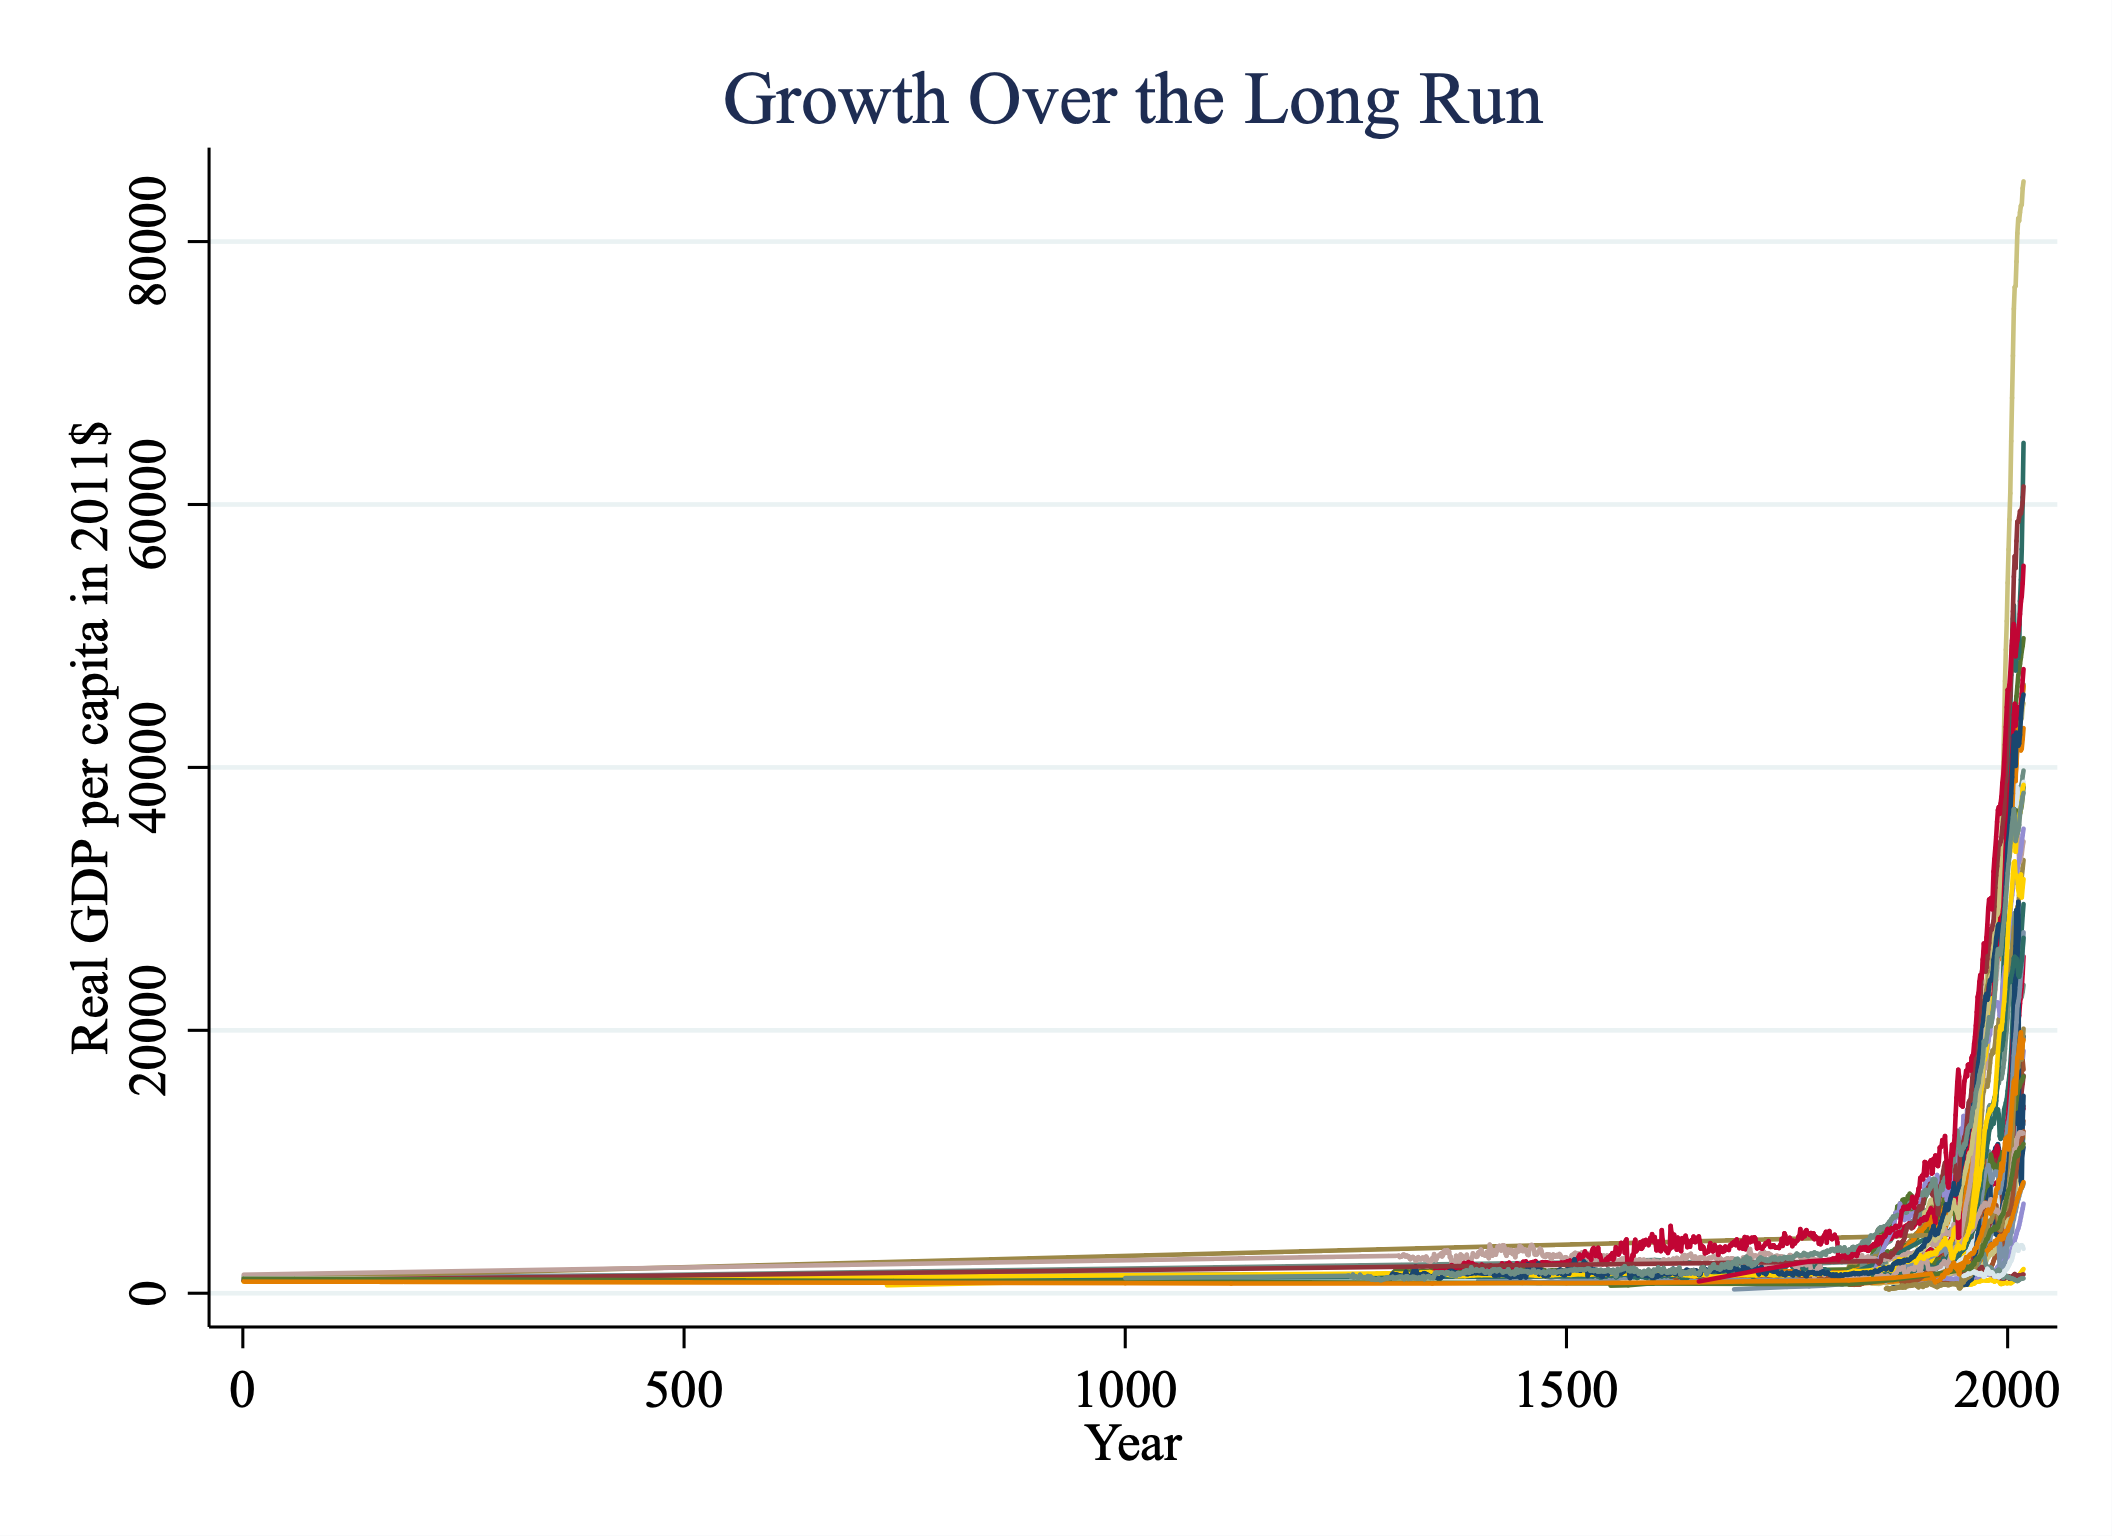
\includegraphics[scale=0.2]{Figures/Fig_7pt0a.png}
\end{figure}
Growth is positively correlated with investment
\end{frame}

\begin{frame}
\frametitle[alignment=center]{As did disparities between countries}
\begin{figure}
\centering
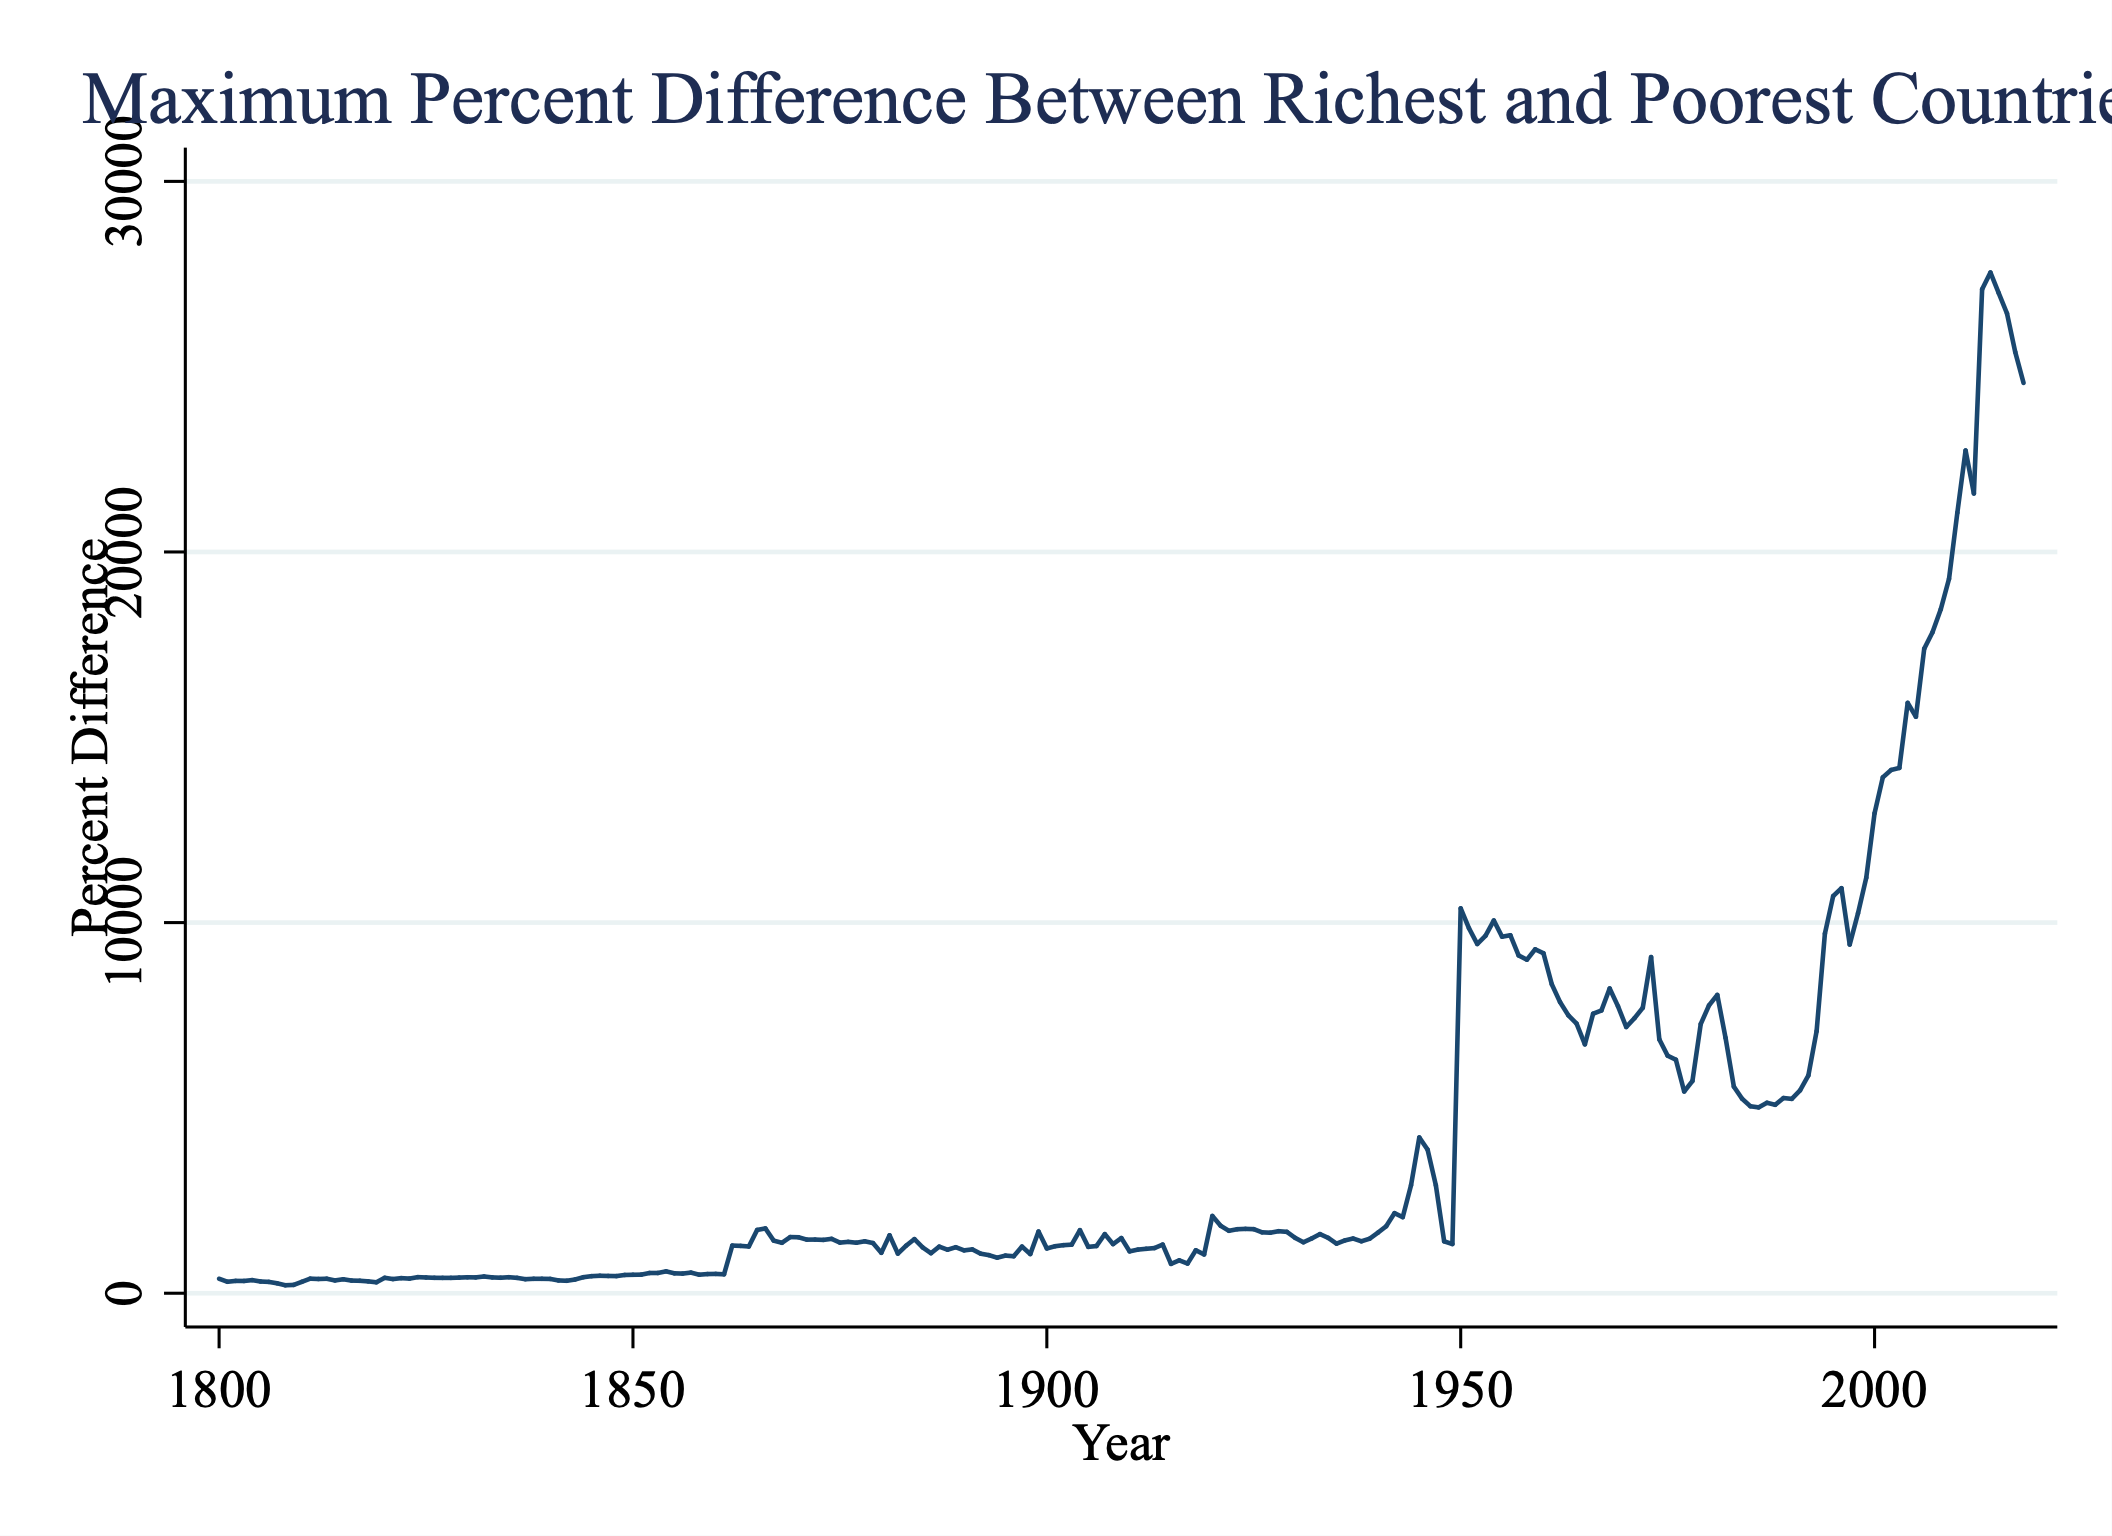
\includegraphics[scale=0.25]{Figures/Fig_7pt0b.png}
\end{figure}
Growth is positively correlated with investment
\end{frame}

\begin{frame}
\frametitle[alignment=center]{Though almost all countries have grown}
\begin{figure}
\centering
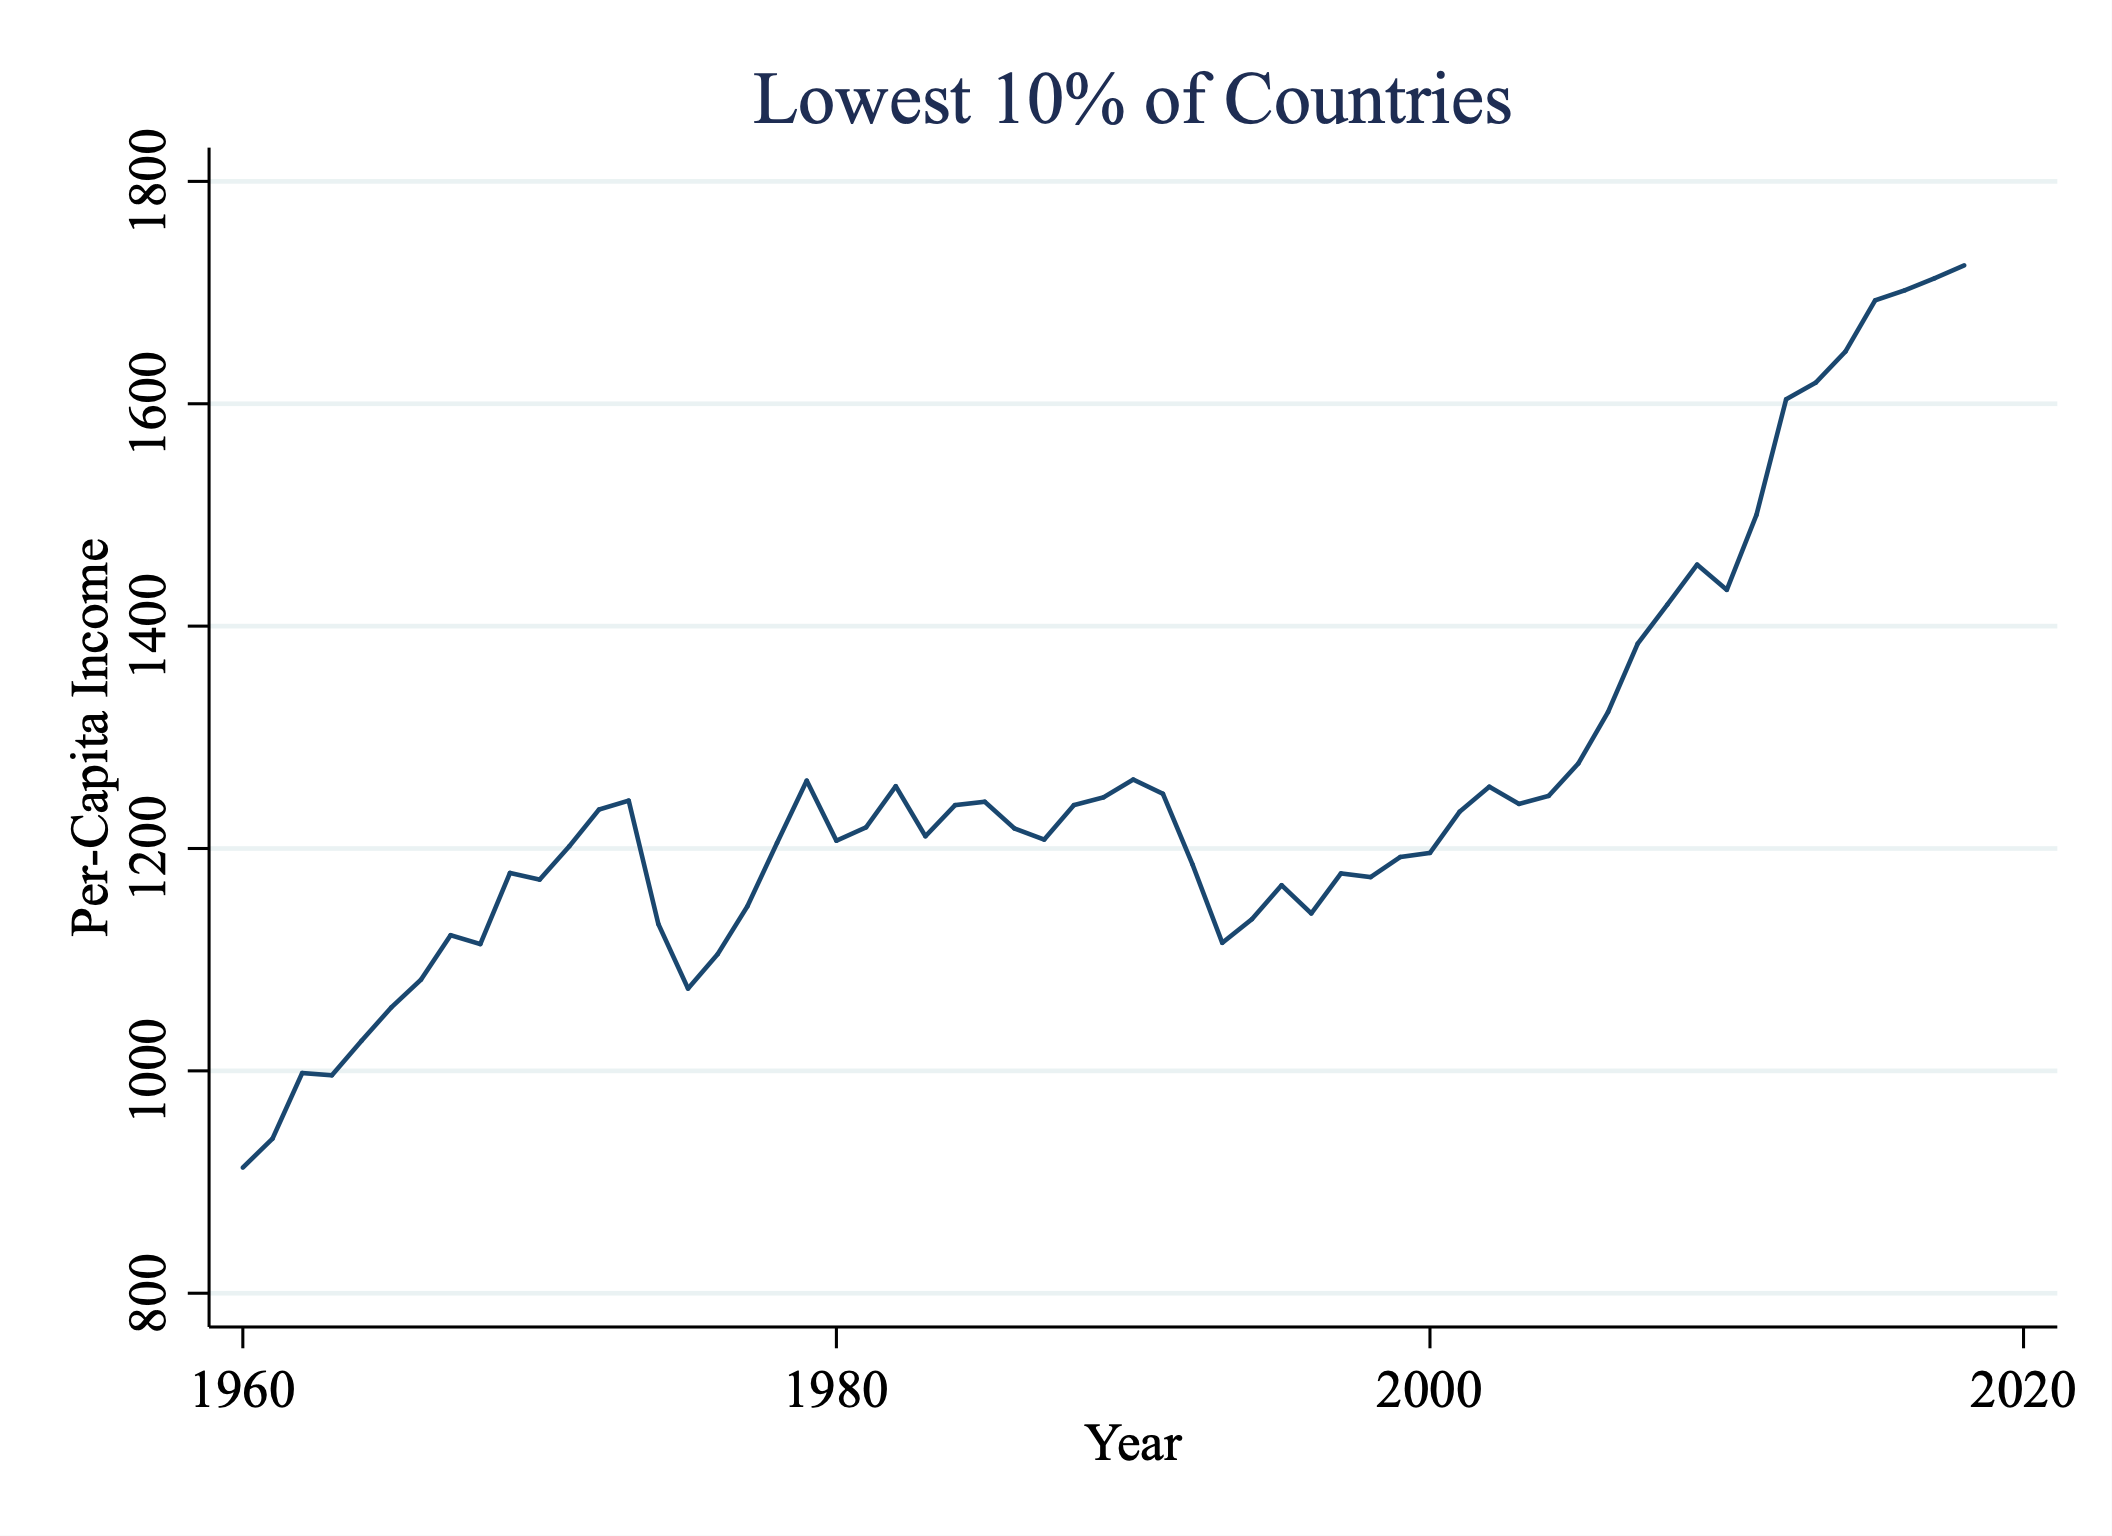
\includegraphics[scale=0.25]{Figures/Fig_7pt0c.png}
\end{figure}
Growth is positively correlated with investment
\end{frame}


\begin{frame}
\frametitle[alignment=center]{Growth is positively correlated with investment}
\begin{figure}
\centering
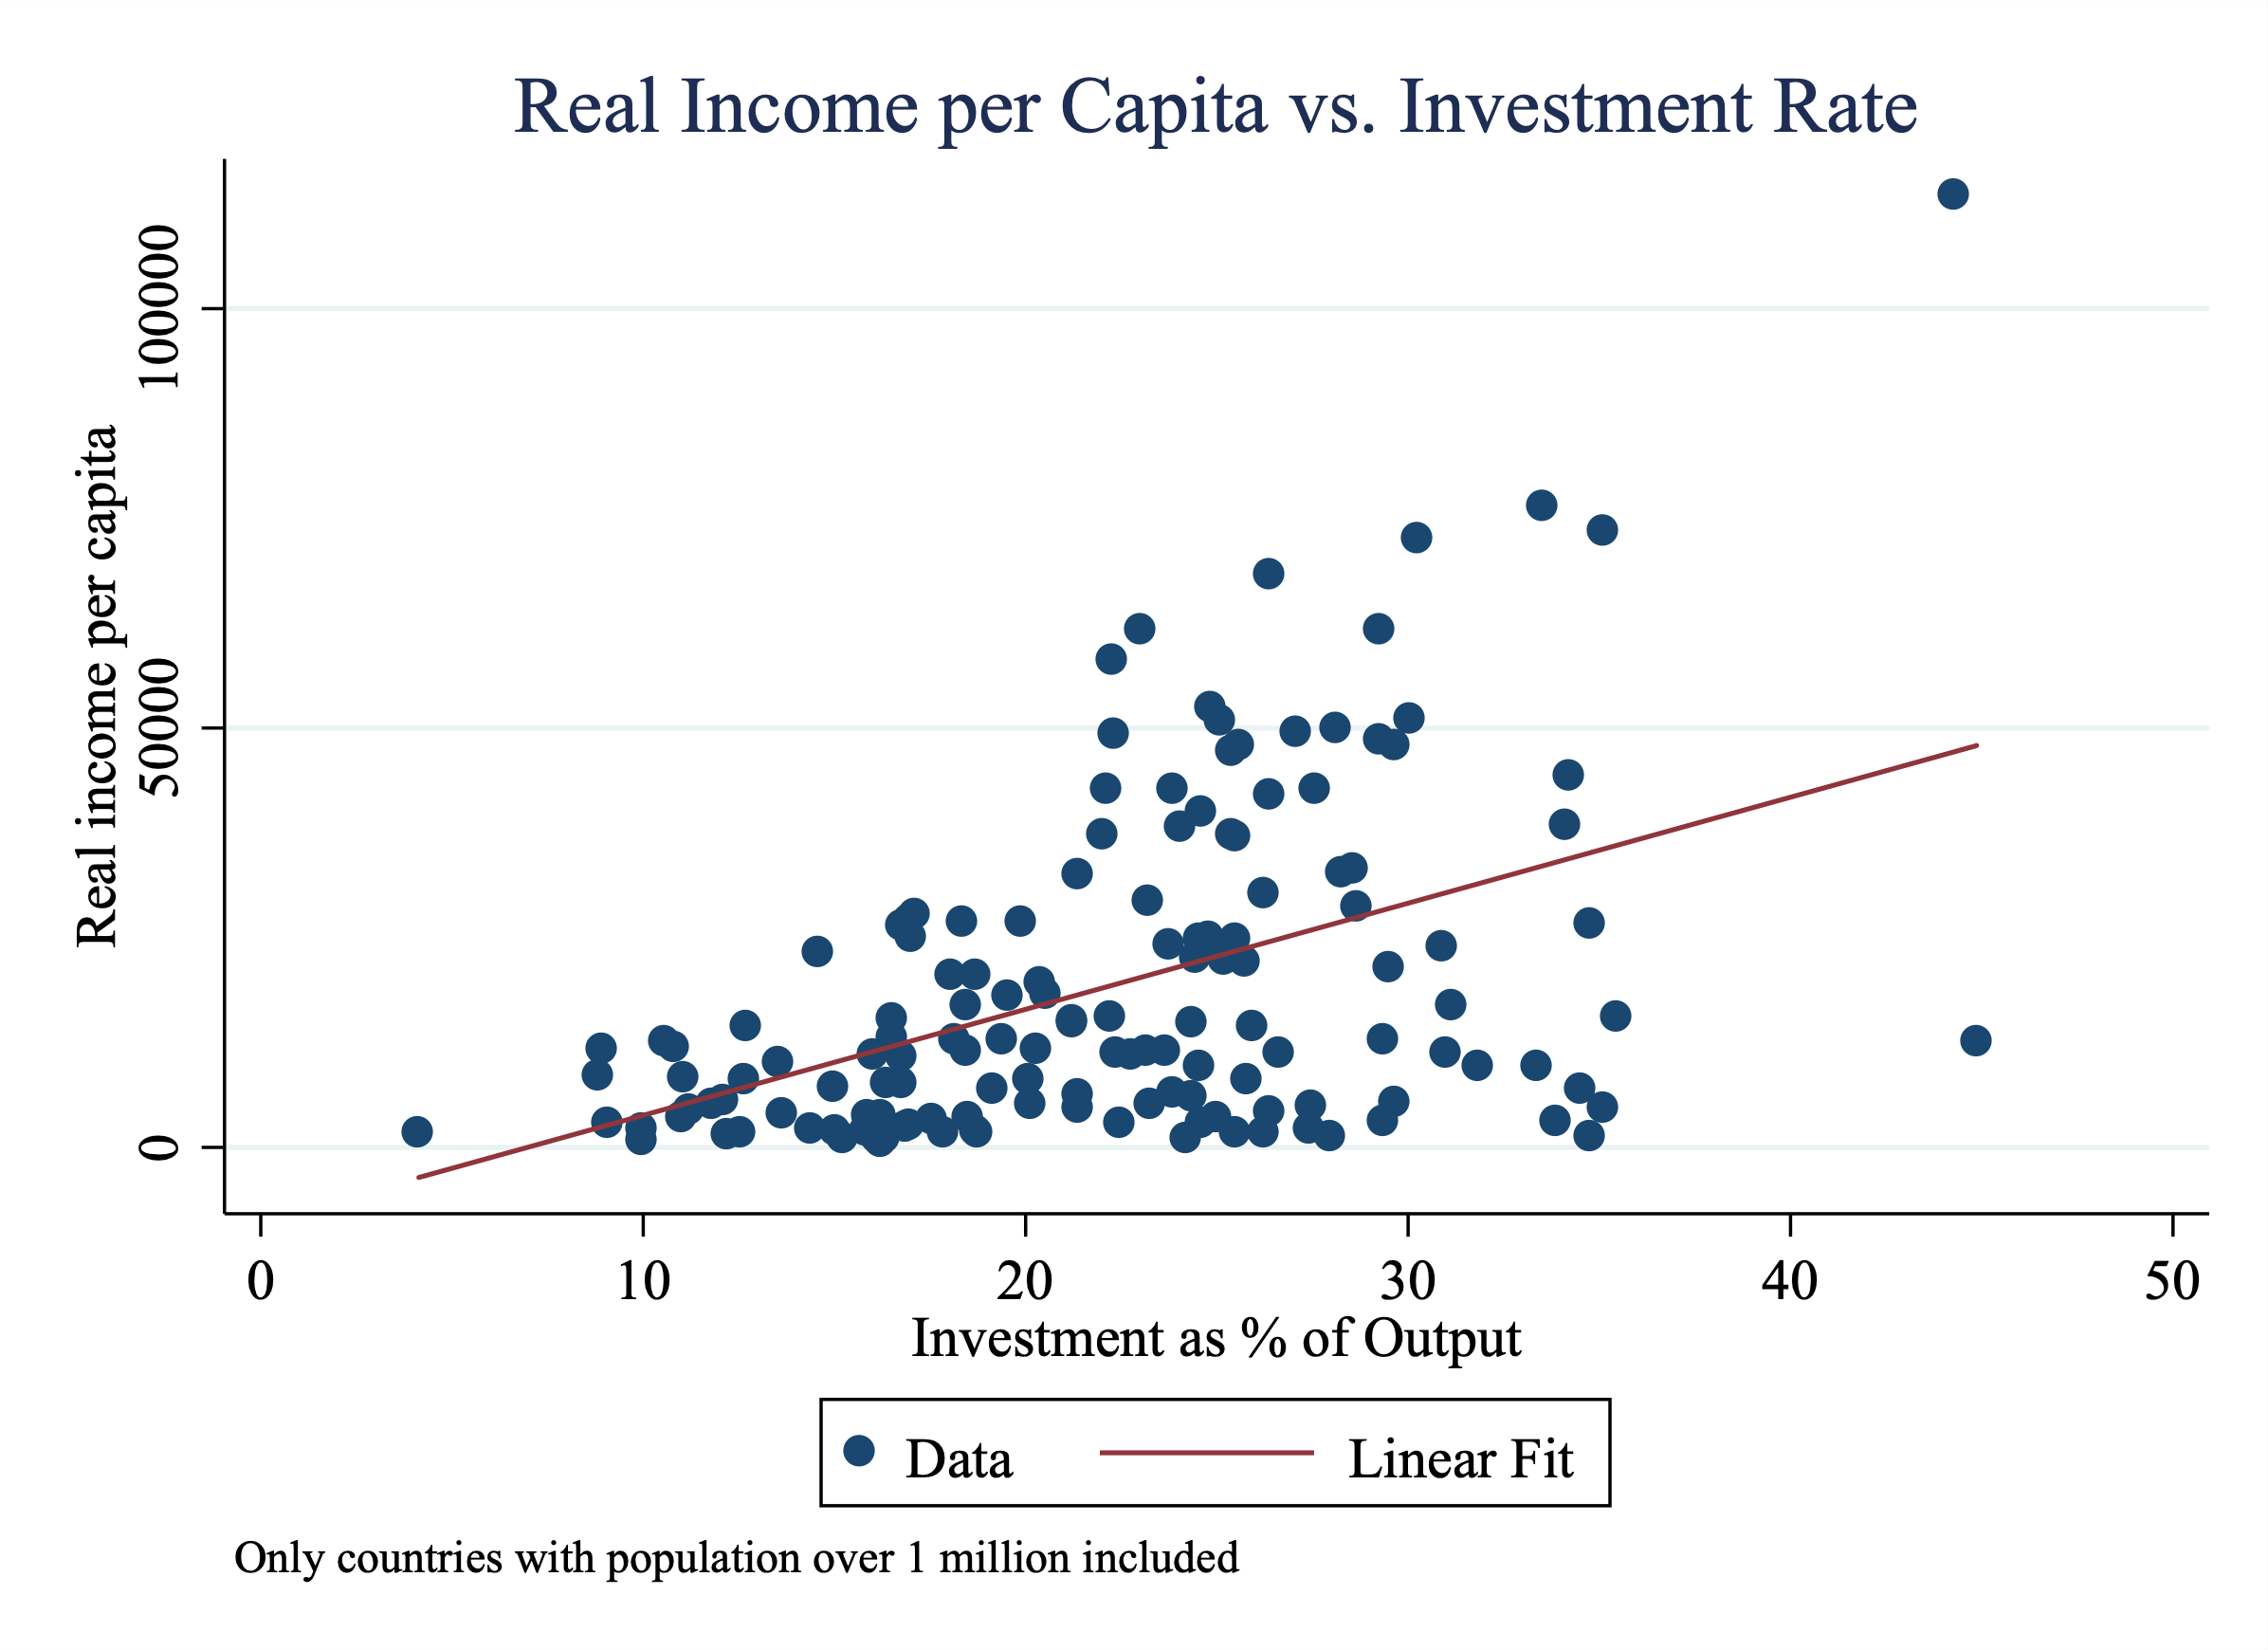
\includegraphics[scale=0.25]{Figures/Fig_7pt1.png}
\end{figure}

\end{frame}

\begin{frame}
\frametitle[alignment=center]{Growth is negatively correlated with population growth}
\begin{figure}
\centering
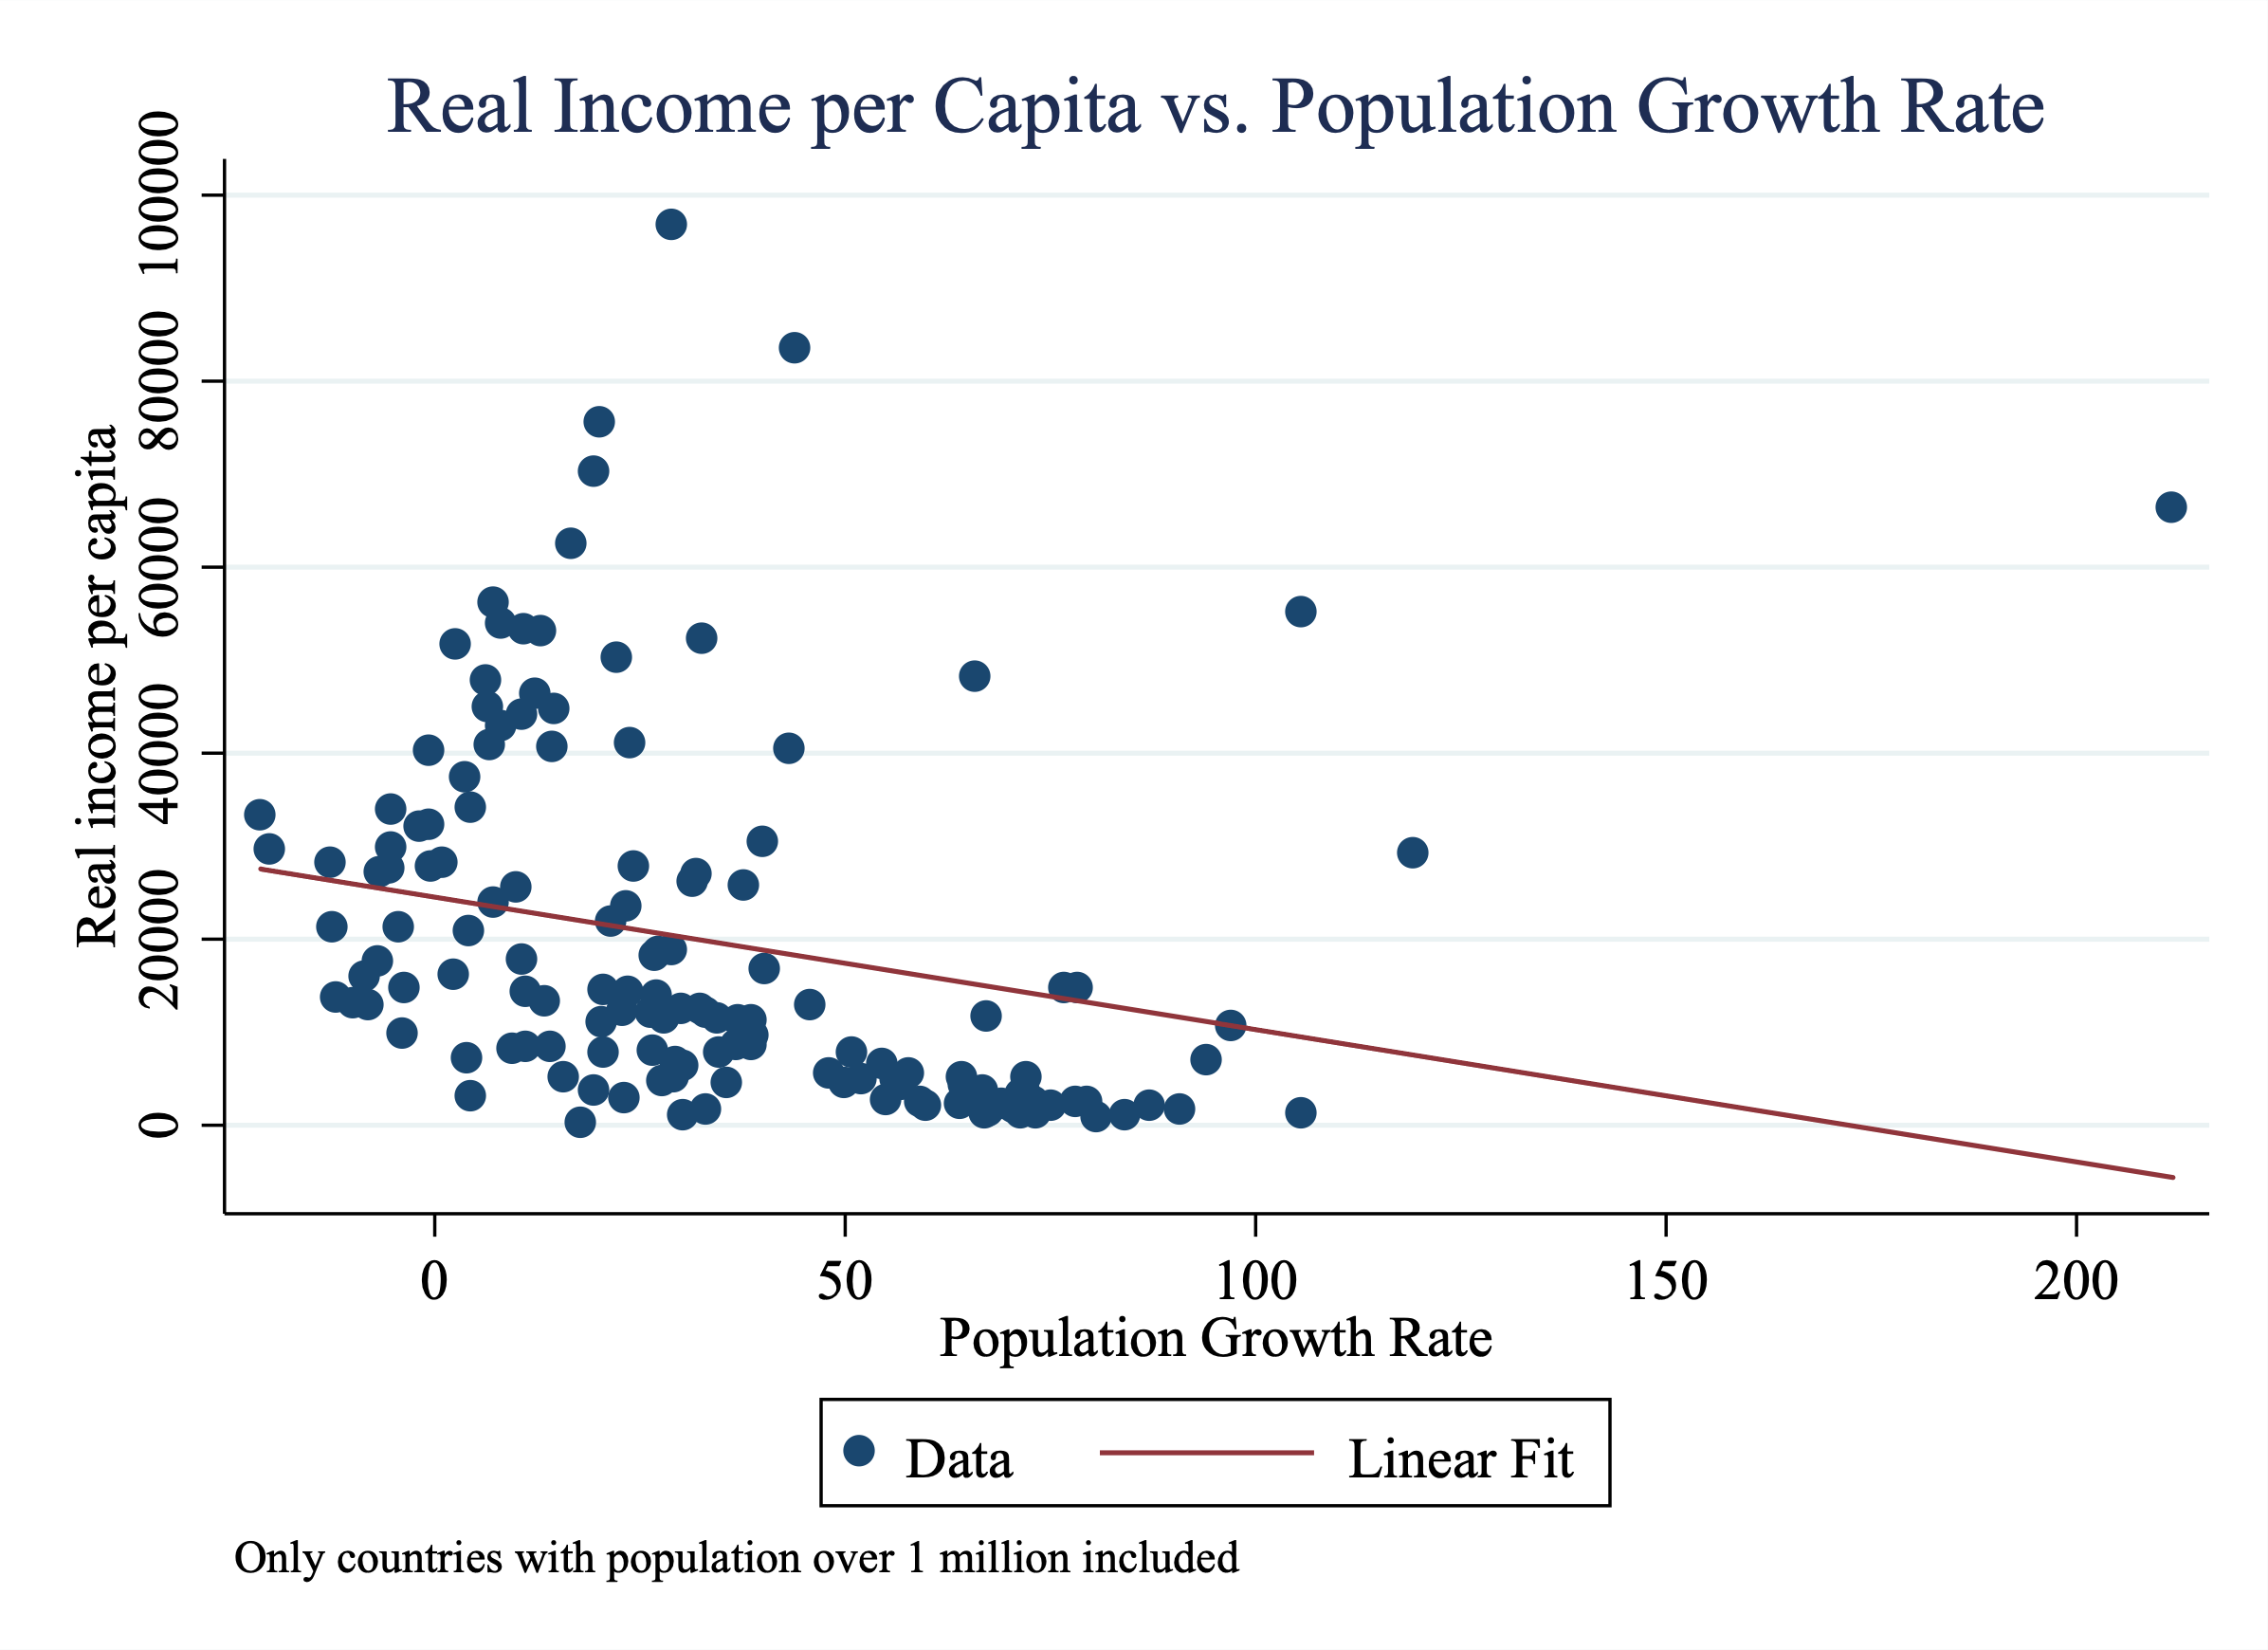
\includegraphics[scale=0.25]{Figures/Fig_7pt2.png}
\end{figure}

\end{frame}

\begin{frame}
\frametitle[alignment=center]{Growth is uncorrelated with initial level of GDP}
\begin{figure}
\centering
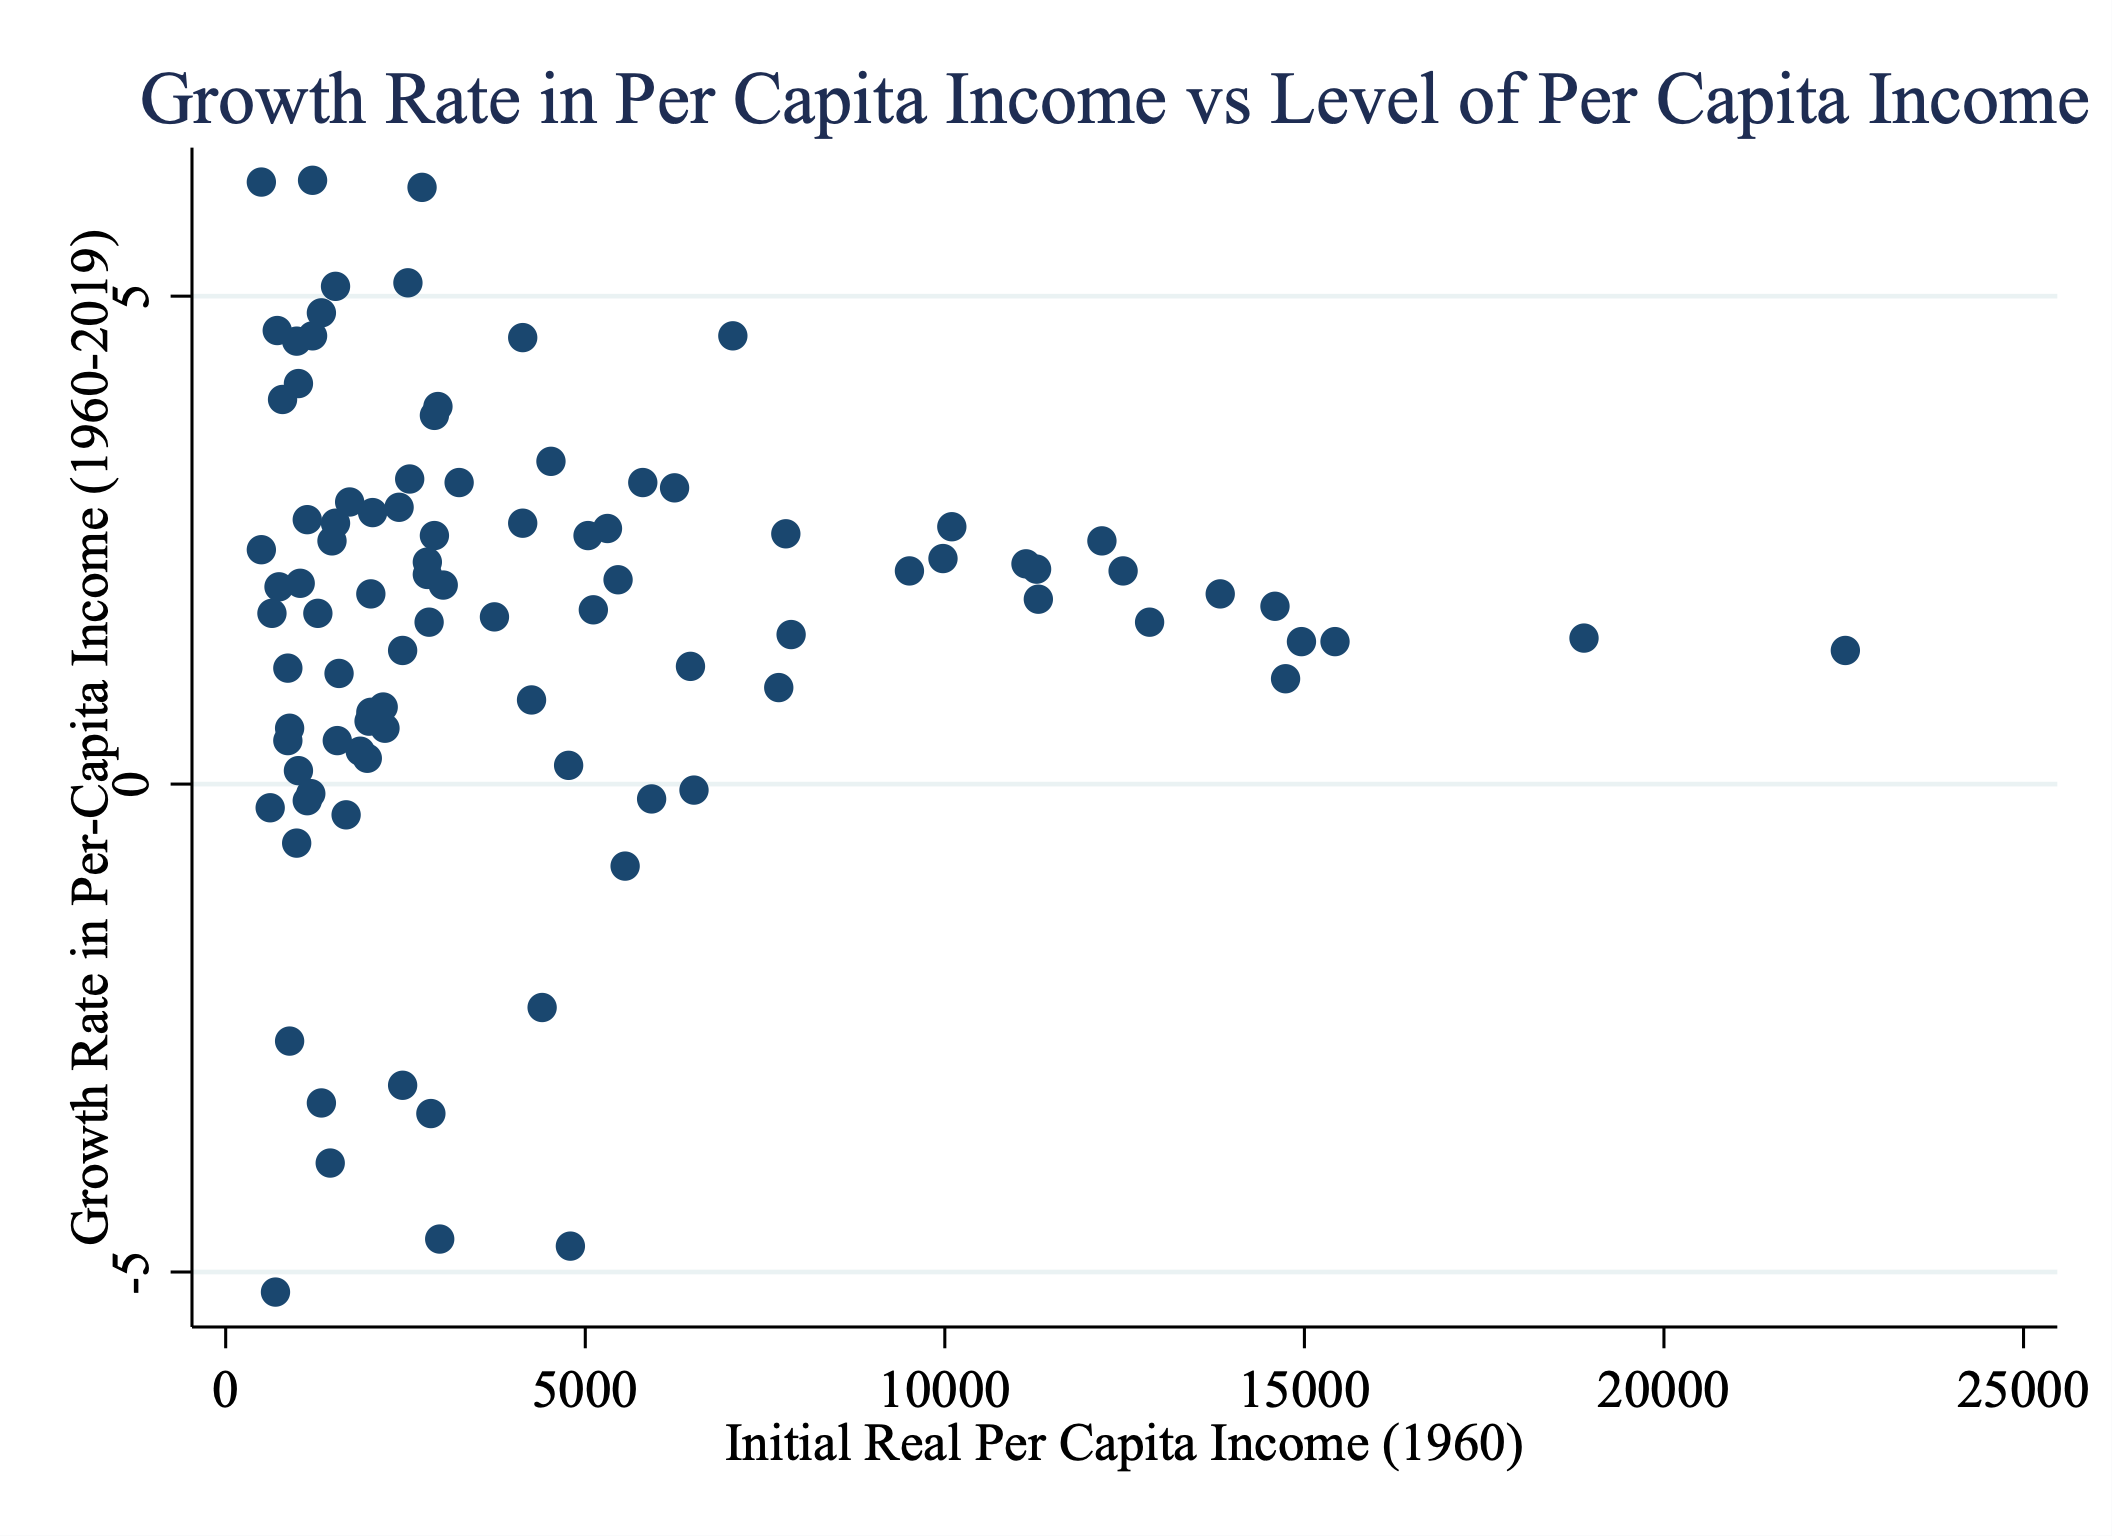
\includegraphics[scale=0.25]{Figures/Fig_7pt3.png}
\end{figure}
 (And is more homogenous among rich countries)
\end{frame}

\begin{frame}
\frametitle[alignment=center]{Growth is uncorrelated with initial level of GDP}
\begin{figure}
\centering
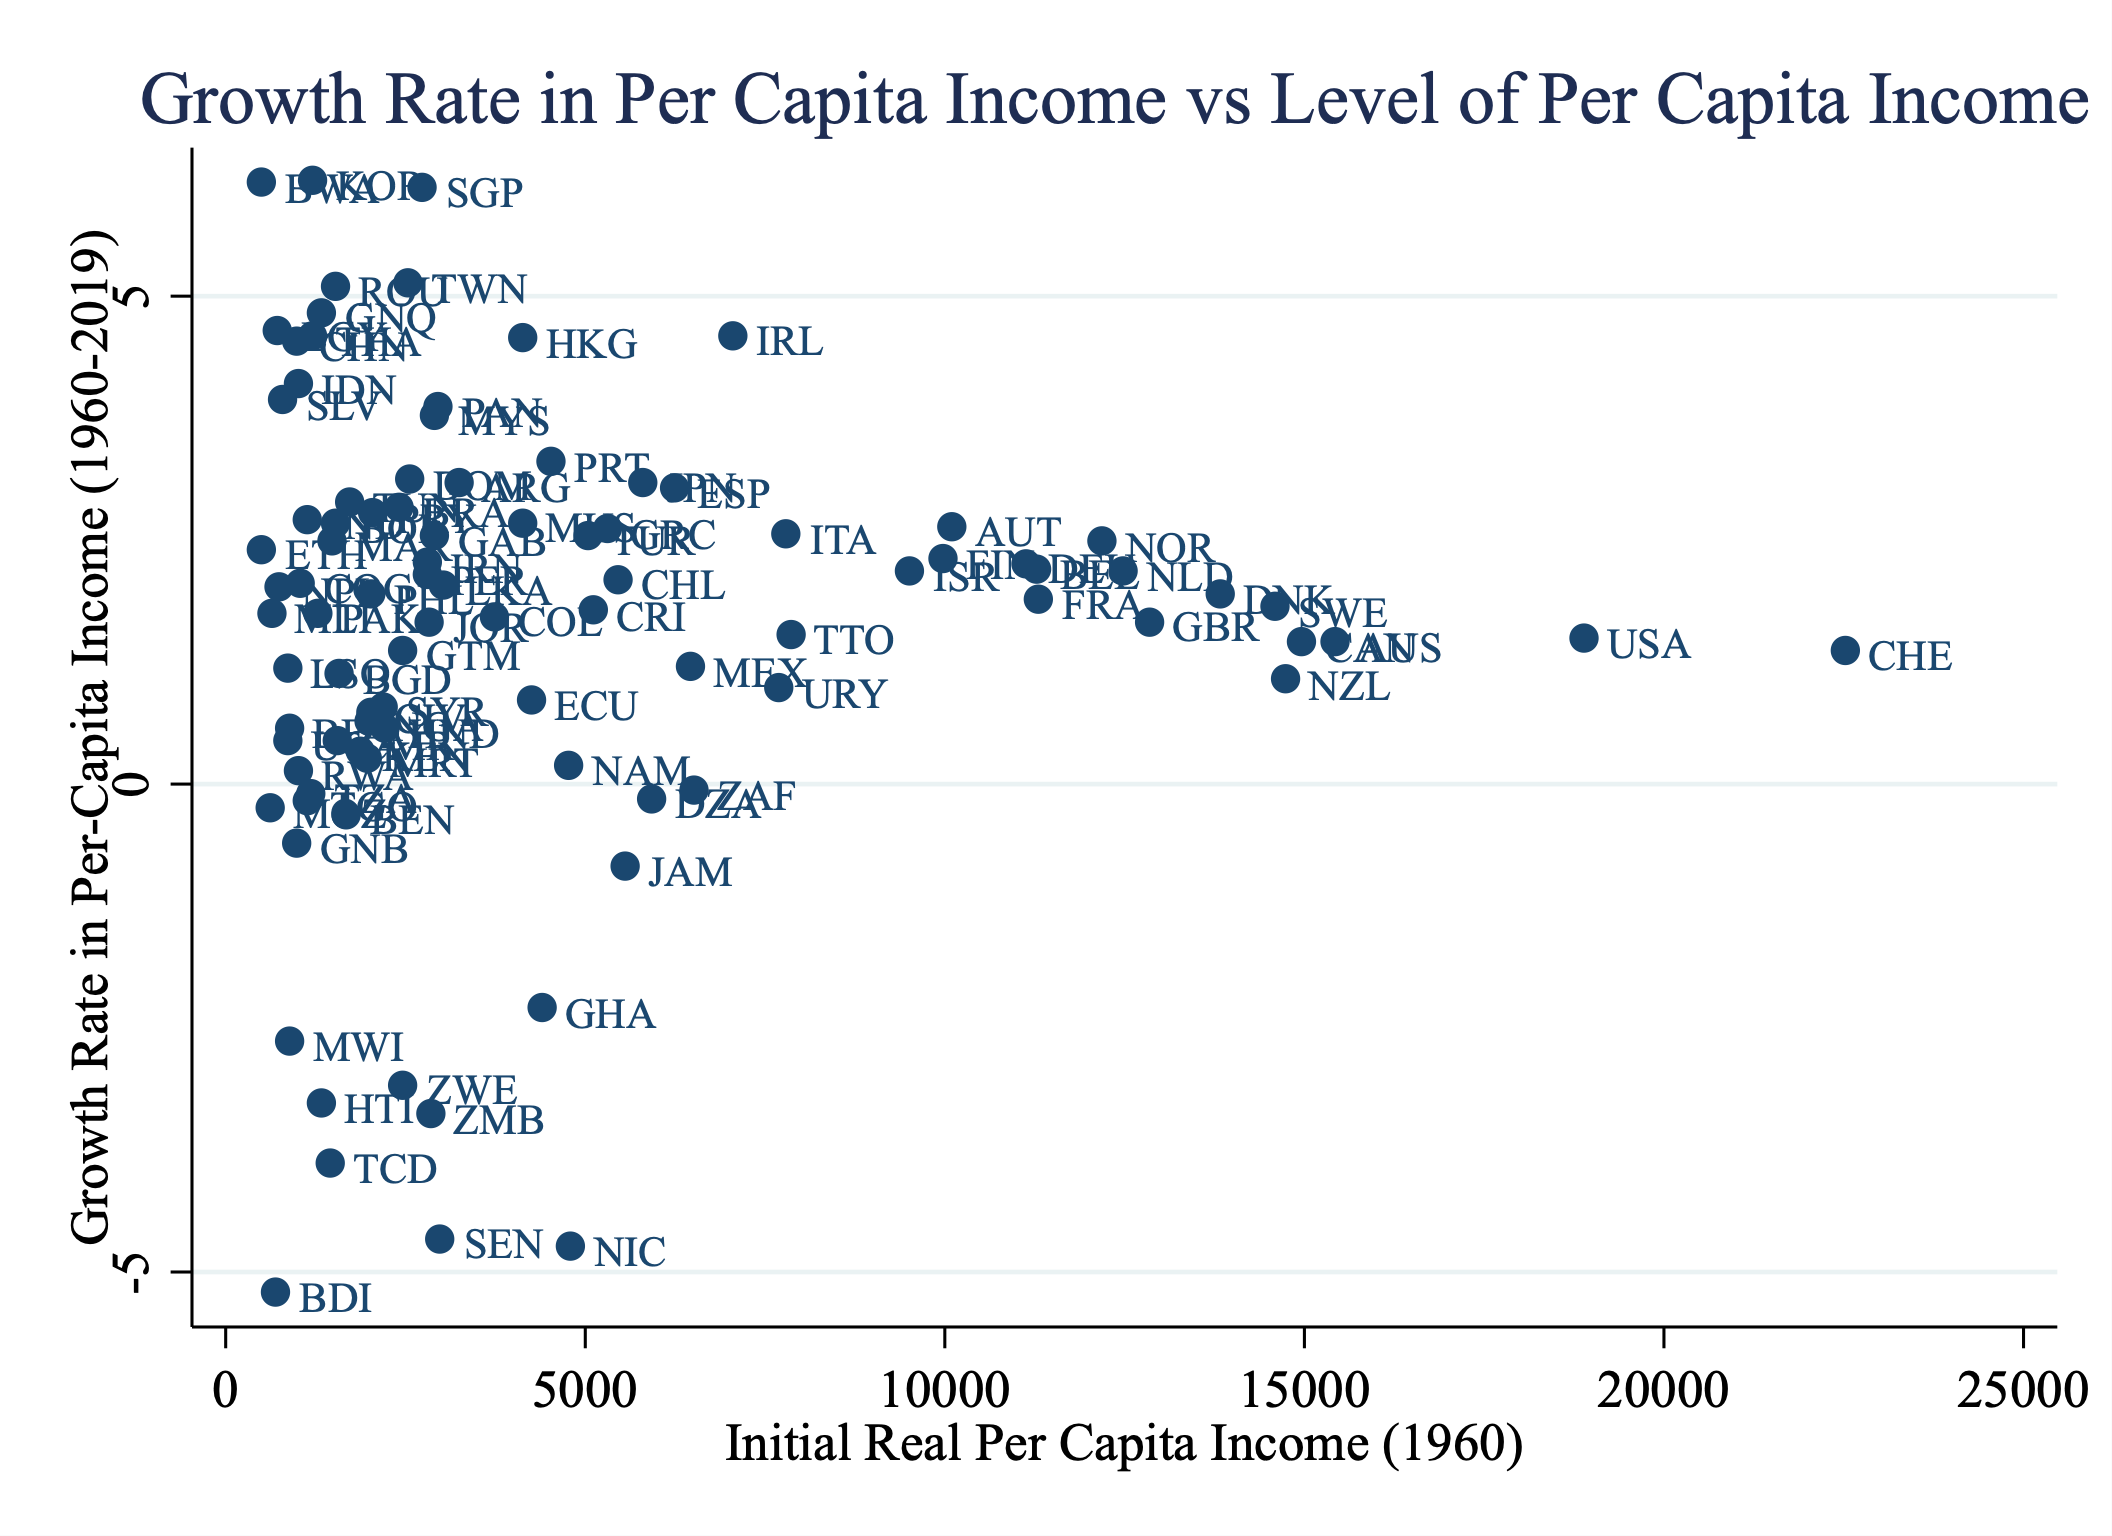
\includegraphics[scale=0.25]{Figures/Fig_7pt3a.png}
\end{figure}
\end{frame}

\begin{frame}
\frametitle[alignment=center]{Malthusian Model of Economic Growth-I}
\begin{itemize}
\item This will be our first model, and it will be terrible
\bigskip
\item Production function $Y$ in terms of TFP $z$, capital (land!) $L$, and labor $N$:
$$Y=zF(L,N)$$
\item Population growth (prime denotes next period):
$$N'=N+\text{Births}-\text{Deaths}$$
\item Or:
$$N'=N+N(\text{birth rate}-\text{death rate})$$
\item But the birth rate, we'll assume, is increasing in consumption per capita $C/N$ (more food, more babies!)
$$\frac{N'}{N}=g\left(\frac{C}{N}\right)$$
\item So need to think about $C/N$
\end{itemize}
\end{frame}

\begin{frame}
\frametitle[alignment=center]{Malthusian Model of Economic Growth-II}
$$C=zF(L,N)$$
\begin{itemize}
\item Or:
$$N'=g\left(zF\left(\frac{L}{N},1\right)\right)N$$
\item Population next period is a concave function of per-capita consumption 
\end{itemize}
\end{frame}


\begin{frame}
\frametitle[alignment=center]{Population Growth in the Steady State}
\begin{figure}
\centering
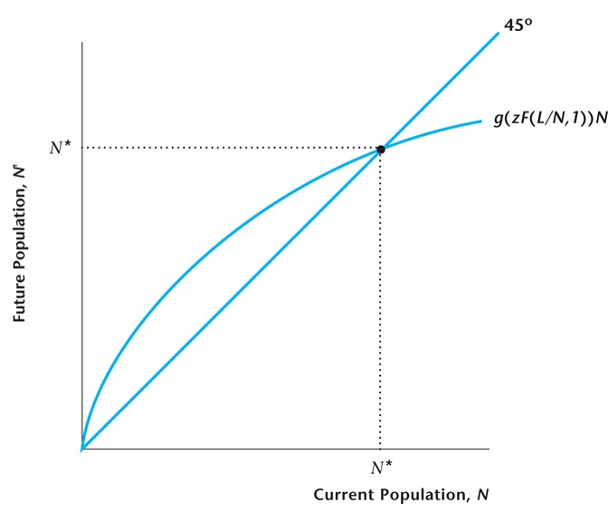
\includegraphics[scale=0.5]{Figures/W_Fig_7pt6.png}
\end{figure}
Consumption has a fixed point!
\end{frame}

\begin{frame}
\frametitle[alignment=center]{Per-Worker Production Function}
\begin{figure}
\centering
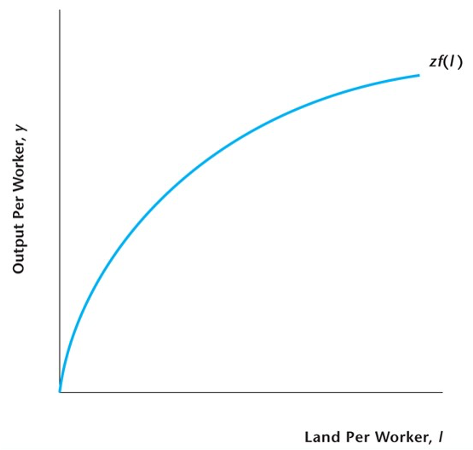
\includegraphics[scale=0.5]{Figures/W_Fig_7pt7.png}
\end{figure}
$$\frac{F(L,N)}{N}=F\left(\frac{L}{N},1\right)=f(l)$$
\end{frame}

\begin{frame}
\frametitle[alignment=center]{Malthusian Model Steady State}
\begin{figure}
\centering
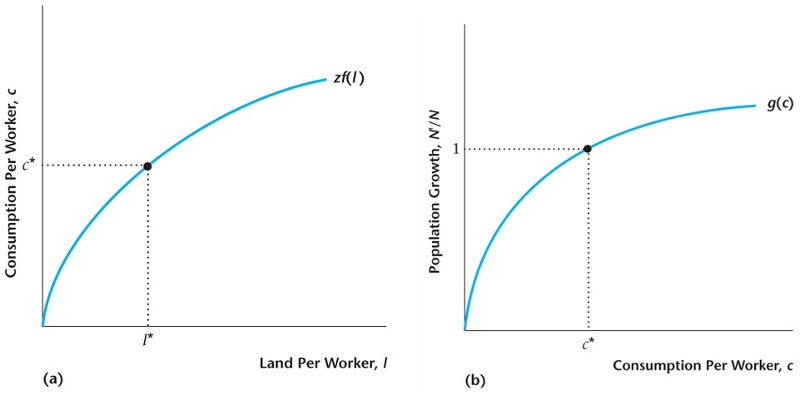
\includegraphics[scale=0.5]{Figures/W_Fig_7pt8.png}
\end{figure}
Now we can analyze shocks to the model: $z$ and population control
\end{frame}

\begin{frame}
\frametitle[alignment=center]{Malthusian Model Equilibrium Intuition}
\begin{itemize}
\item What are these equations/this model telling us?
\bigskip
\item We assume:
\smallskip
\begin{enumerate} 
\item land is fixed
\smallskip
\item  production as a function of labor alone is decreasing returns
\smallskip
\item population growth depends on consumption
\end{enumerate}
\smallskip
\item Then if there aren't many people, they're very productive!  Consumption is high, more children, consumption falls, still more children, until consumption falls enough that there is no more growth to the steady state
\bigskip
\item Reverse if too many people:  population growth goes negative, people grow more productive, and we converge from above to the steady state
\bigskip
\item Now let's analyze what happens with an increase in total factor productivity $(z)$ and how population control would work
\end{itemize}
\end{frame}




\begin{frame}
\frametitle[alignment=center]{Increase in $z$}
\begin{figure}
\centering
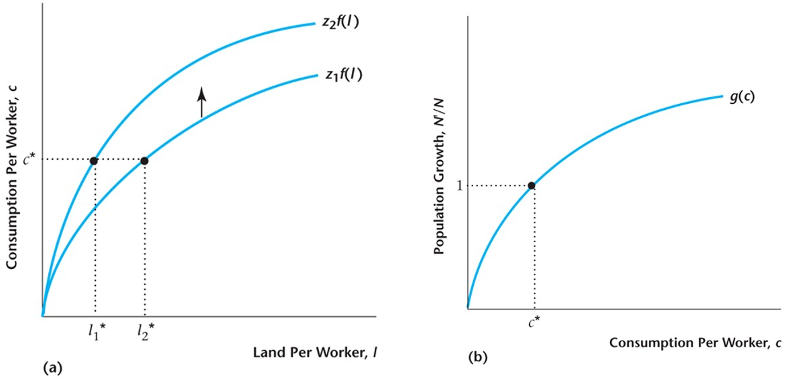
\includegraphics[scale=0.5]{Figures/W_Fig_7pt9.png}
\end{figure}
\end{frame}



\begin{frame}
\frametitle[alignment=center]{Increase in $z$}
\begin{figure}
\centering
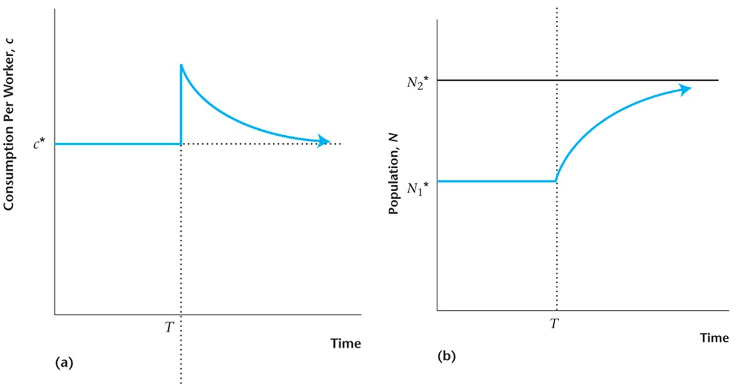
\includegraphics[scale=0.5]{Figures/W_Fig_7pt10.png}
\end{figure}
\end{frame}

\begin{frame}
\frametitle[alignment=center]{Population Control}
\begin{figure}
\centering
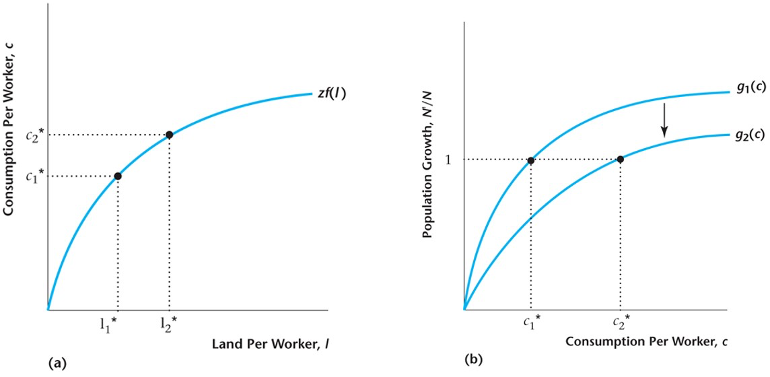
\includegraphics[scale=0.5]{Figures/W_Fig_7pt11.png}
\end{figure}
\end{frame}


\begin{frame}
\frametitle[alignment=center]{Is the Malthusian model any good?}
\begin{itemize}
\item No!  It's truly terrible
\bigskip
\begin{itemize}
\item Aside: people aren't animals!  There is \textbf{no} boom in babies after power-outs, \textbf{no} increase in births due to lockdowns.  Every M.D. or nurse I've ever talked to about this gets this badly wrong! ($N>8$)
\end{itemize}
\bigskip
\item But it's a start on modellng growth
\bigskip
\item Main change:  land may be fixed, but capital isn't!  
\bigskip
\item Also, income and population growth are negatively correlated (at the country and the individual level)
\bigskip
\item Issues with assumptions, but method/idea seems sound
\end{itemize}
\end{frame}

\begin{frame}
\frametitle[alignment=center]{Population Growth by Country}
\begin{figure}
\centering
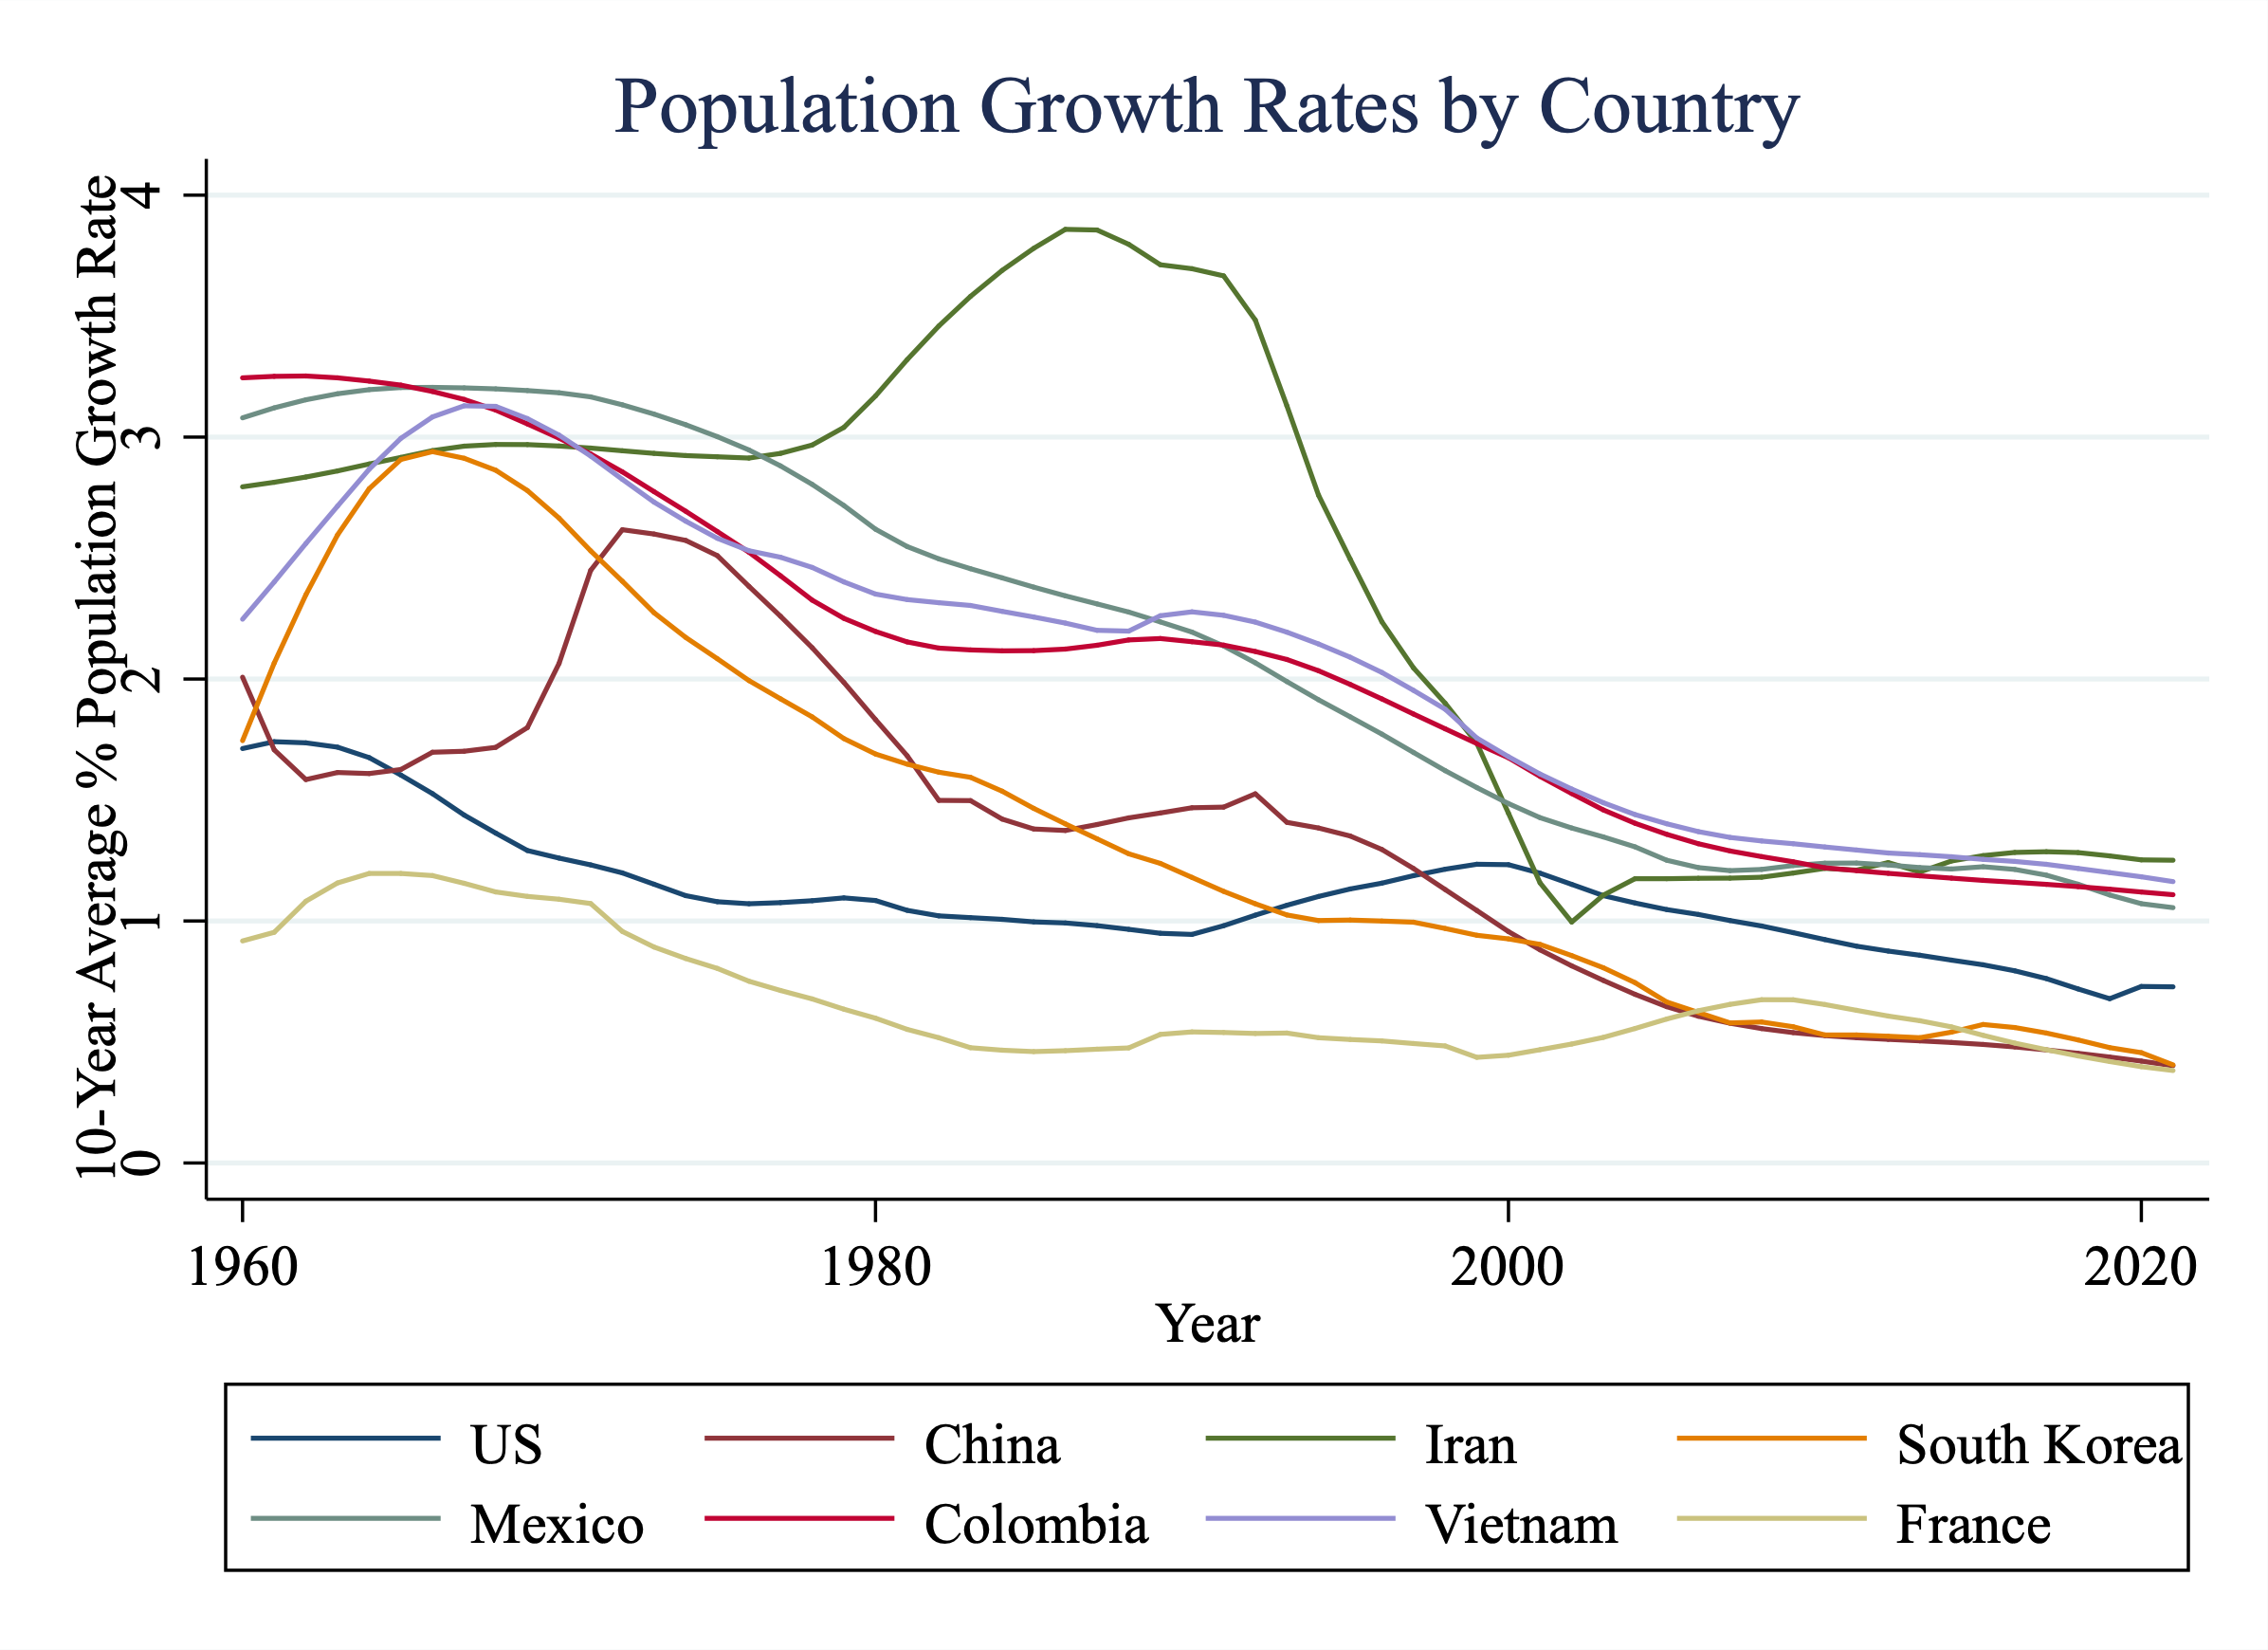
\includegraphics[scale=0.25]{Figures/PopGrowth_country.png}
\end{figure}
\end{frame}


\begin{frame}
\frametitle[alignment=center]{Population Growth by Region}
\begin{figure}
\centering
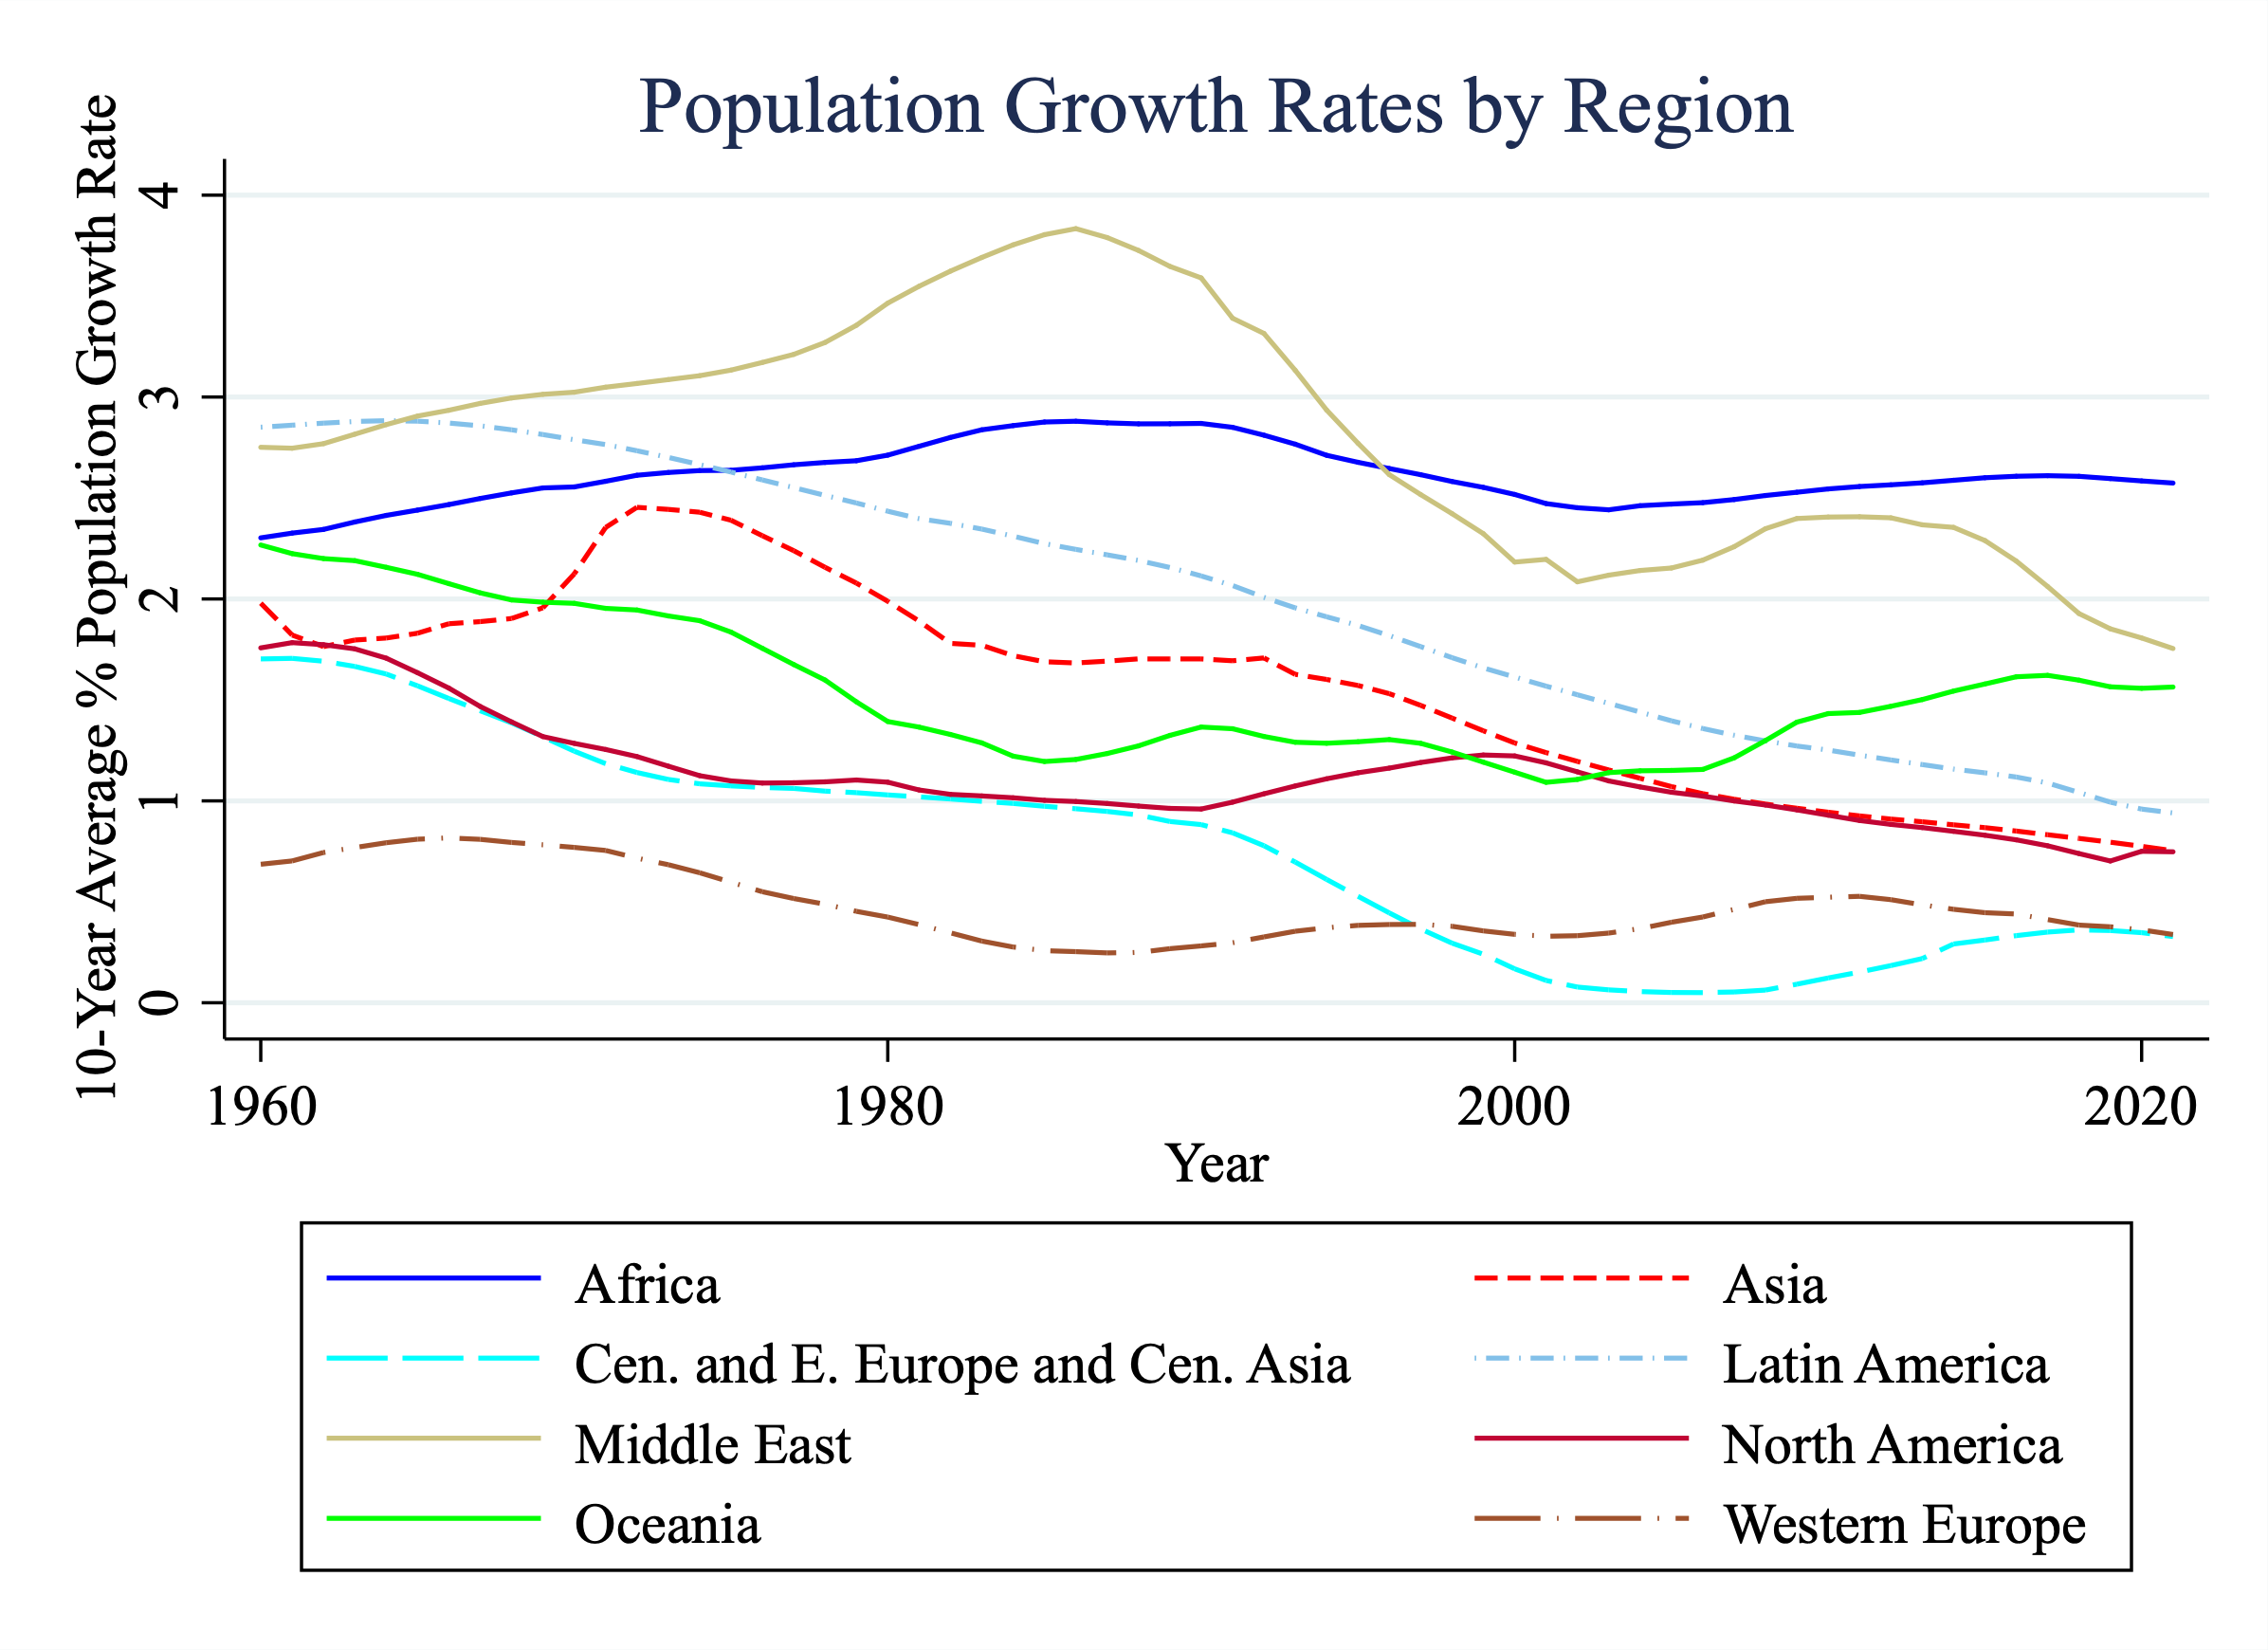
\includegraphics[scale=0.25]{Figures/PopGrowth_region.png}
\end{figure}
\end{frame}

\begin{frame}
\frametitle[alignment=center]{Solow Growth Model-Overview}
\begin{itemize}
\item We need a better model of growth than Malthusian
\bigskip
\item What's the name of the game since 1800?  Increasing productivity ($z$)!
\bigskip
\item Let's say $z$ is exogenously increasing (changing), human knowledge grows
\bigskip
\item Population growth is fixed
\bigskip
\item Savings/consumption are just constant fractions of production  (simple assumption)
\bigskip
\item Let it rip
\end{itemize}
\end{frame}


\begin{frame}
\frametitle[alignment=center]{Solow Growth Model-I}
\begin{itemize}
\item Assumption 1: Population growth:
$$N'=(1+n)N$$
\item Assumption 2: $s$ is (constant) fraction of product saved, $1-s$ is fraction consumed
$$C=(1-s)Y$$
\item Assumption 3: Firms face the production function:
$$Y=zF(K,N)$$
\item Or in per-capita terms, because CRS:
$$y=zf(k)$$
\item Assumption 4: Capital has a law of motion:
$$K'=(1-\delta)K+I$$
\item Assumption 5:  feasibility/social planner budget constraint:
$$Y=C+I$$
\end{itemize}
\end{frame}

\begin{frame}
\frametitle[alignment=center]{Solow Growth Model-II}
\begin{itemize}
\item \item Now we can solve for growth and the ``steady state" like we did with Malthus.  Start with Assumption 5: 
$$Y=C+I$$
\item Solving for $I$ in Assumption 4 and plugging in:
$$K'=sY+(1-\delta)K$$
\item Using Assumption 3 and dividing by $N$:
$$\frac{K'}{N}=sz\frac{F(K,N)}{N}+(1-\delta)\frac{K}{N}$$
\item Multiplying and dividing by $N'$, we get in per-capita terms:
$$k'(1+n)=szf(k)+(1-\delta)k$$
\item Or:
$$k'=\frac{szf(k)}{1+n}+\frac{(1-\delta)k}{1+n}$$
\item Now we have how capital moves as a function of capital, can graph for equilibrium
\end{itemize}
\end{frame}


\begin{frame}
\frametitle[alignment=center]{Determination of the Steady State Quantity of Capital Per Worker}
\begin{figure}
\centering
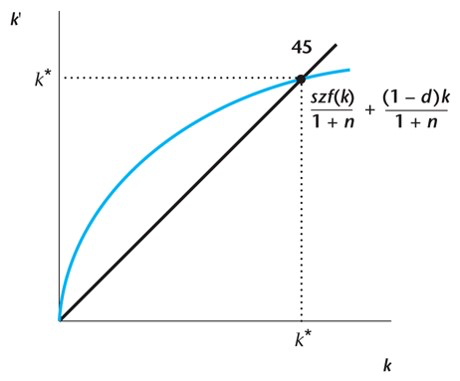
\includegraphics[scale=0.5]{Figures/W_Fig_7pt13.png}
\end{figure}
\end{frame}

\begin{frame}
\frametitle[alignment=center]{Analyzing the Steady State}
\begin{itemize}
\item In the steady state, $k^*=k'=k$, so:
$$k^*=\frac{szf(^*)}{1+n}+\frac{(1-\delta)^*}{1+n}$$
\item Or:
$$szf(k^*)=(n+\delta)k^*$$
\item With this, we can ask:  what happens to $k^*$ when $n$, $\delta$, $s$, or $z$ increase?
\bigskip
\item Also note that $c^*=(1-s)y^*=(1-s)zf(k^*)$, so this also tells us about consumption
\bigskip
\item The advantage is this will tell us what could and could not be causing growth!
\end{itemize}
\end{frame}



\begin{frame}
\frametitle[alignment=center]{Determination of the Steady State Quantity of Capital Per Worker}
\begin{figure}
\centering
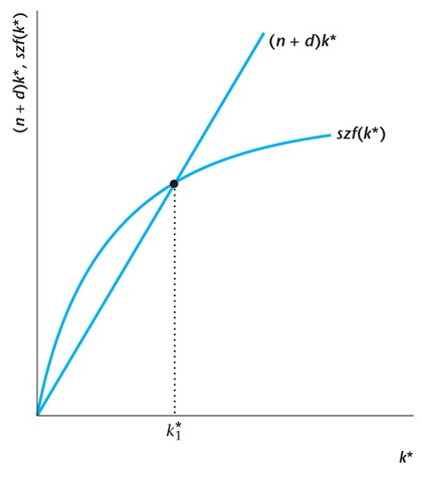
\includegraphics[scale=0.5]{Figures/W_Fig_7pt14.png}
\end{figure}
\end{frame}

\begin{frame}
\frametitle[alignment=center]{Increase in Savings Increases SS $k^*$}
\begin{figure}
\centering
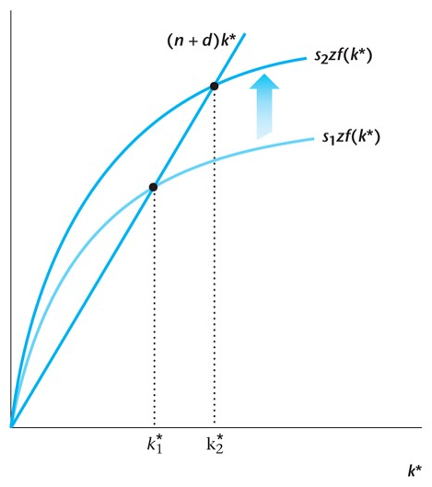
\includegraphics[scale=0.5]{Figures/W_Fig_7pt15.png}
\end{figure}
\end{frame}


\begin{frame}
\frametitle[alignment=center]{Effect of an Increase in the Savings Rate at time T}
\begin{figure}
\centering
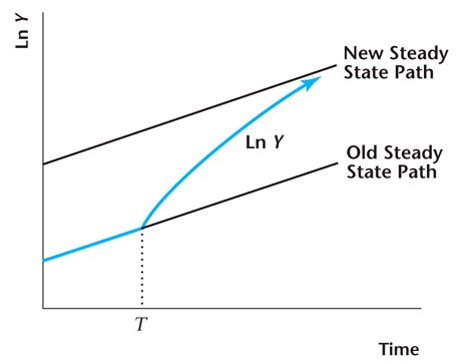
\includegraphics[scale=0.5]{Figures/W_Fig_7pt16.png}
\end{figure}
\end{frame}

\begin{frame}
\frametitle[alignment=center]{Steady State consumption per worker}
\begin{figure}
\centering
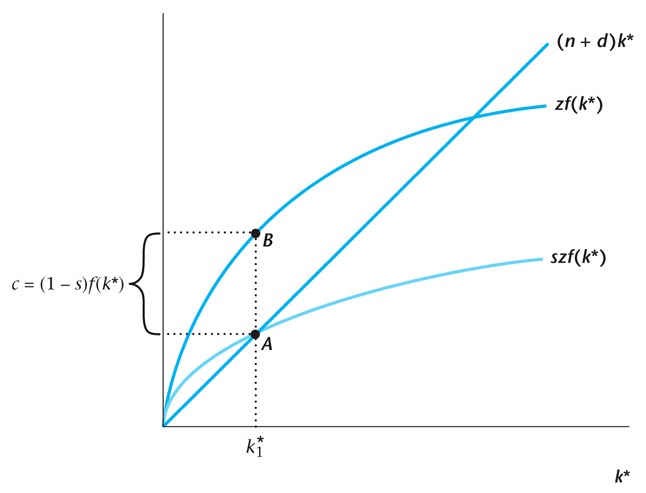
\includegraphics[scale=0.5]{Figures/W_Fig_7pt17.png}
\end{figure}
\end{frame}


\begin{frame}
\frametitle[alignment=center]{Consumption per worker and the Golden Rule Capital Accumulation}
\begin{itemize}
\item What is the ``best" choice of savings rate (asterisk!)
\bigskip
\item Let's maximize consumption $c$ using $s$:  on one hand, when it increases, more $K$, but less $(1-s)Y$
\bigskip
\item Find the maximize
\end{itemize}
\end{frame}


\begin{frame}
\frametitle[alignment=center]{Golden Rule Capital Accumulation}
\begin{itemize}
\item Start with consumption as difference of production minus investment (see previous graph):
$$c=zf(k^*)-(n+\delta)k^*$$
\item Where these two are farthest apart is the optimal (consumption-maximizing) level of capital
\bigskip
\item That's where their slopes are equal! $\frac{\partial zf(k^*)}{\partial z^*}=\frac{\partial (n+\delta)k^*}{\partial k^*}$
\bigskip
\item Or where:
$$MP_K=n+\delta$$
\bigskip
\item Let's plot $s^*zf(k^*)$, $zf(k^*)$ and $(n+\delta)k^*$:  best is when $s^*zf(k^*)$ intersects $(n+\delta)k^*$
\end{itemize}
\end{frame}


\begin{frame}
\frametitle[alignment=center]{Golden Rule Quantity of Capital per Worker}
\begin{figure}
\centering
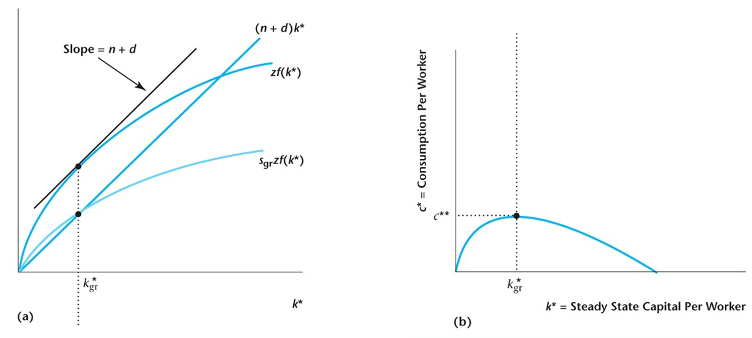
\includegraphics[scale=0.5]{Figures/W_Fig_7pt18.png}
\end{figure}
\end{frame}

\begin{frame}
\frametitle[alignment=center]{Labor Force Growth Rate}
\begin{itemize}
\item What happens to GDP per capita when the labor force starts growing at a permanently higher rate? $(1+n)\rightarrow(1+n')$ where $n'>n$?
\bigskip
\item We can draw it!  
\bigskip
\item But also recall we stop growing when $szf(k^*)=(n+\delta)k^*$
\bigskip
\item If RHS increases because of $n$, then LHS must increase.  How?
\bigskip
\item By decreasing $k^*$!  
\end{itemize}
\end{frame}


\begin{frame}
\frametitle[alignment=center]{Steady State Effects of an Increase in Labor Force Growth Rate}
\begin{figure}
\centering
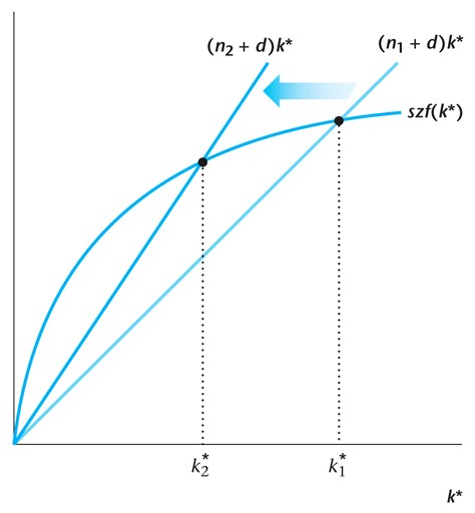
\includegraphics[scale=0.5]{Figures/W_Fig_7pt19.png}
\end{figure}
\end{frame}

\begin{frame}
\frametitle[alignment=center]{Steady State Effects of an Increase in Productivity}
\begin{figure}
\centering
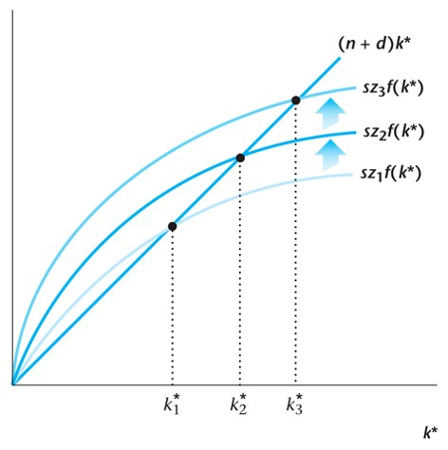
\includegraphics[scale=0.5]{Figures/W_Fig_7pt20.png}
\end{figure}
\end{frame}


\begin{frame}
\frametitle[alignment=center]{Measuring Z}
\begin{itemize}
\item How can we measure $z$?
\bigskip
\item Our model can help!
\item Start with the production function:
$$Y=zF(K,N)$$
\item Assume a Cobb-Douglas form:
$$F(K,N)=K^\alpha N^{1-\alpha}$$
\item Put numbers on $\alpha$:
$$Y=zK^{0.3}N^{0.7}$$
\item Then solve for $z$:
$$\hat{z}=\frac{\hat{Y}}{\hat{K}^{0.3}\hat{N}^{0.7}}$$
\end{itemize}
\end{frame}




%\begin{frame}
%\frametitle[alignment=center]{Breaking from Trend}
%\begin{figure}
%\centering
%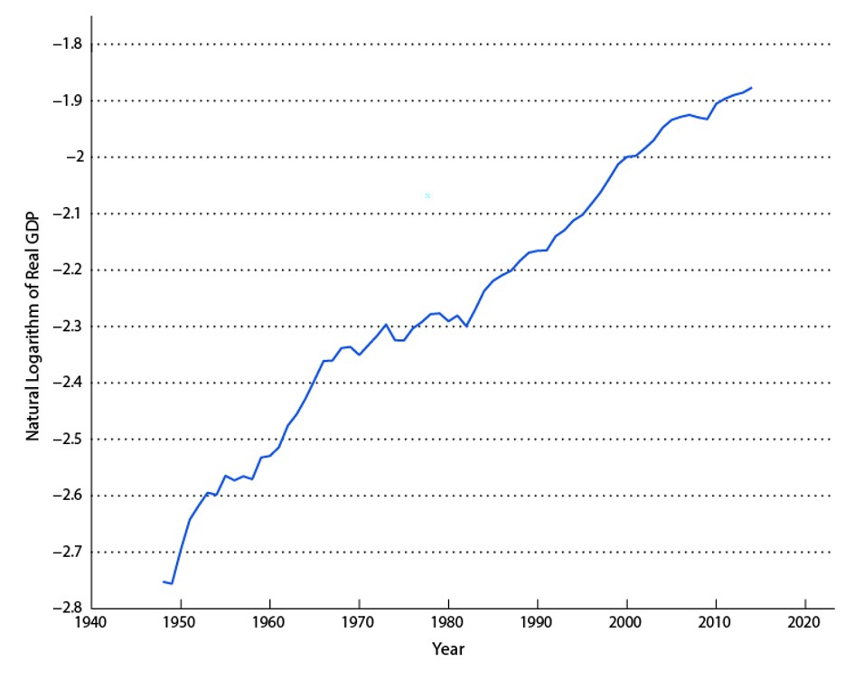
\includegraphics[scale=0.5]{Figures/W_Fig_7pt23.png}
%\end{figure}
%\end{frame}
%
%\begin{frame}
%\frametitle[alignment=center]{Average Annual Growth Rates in the Solow Residual}
%\begin{table}
%\begin{tabular}{lc}
%Years & Average Annual Growth Rate \\
%\hline
%1950-1960 & 1.7\\
%1960-1970 & 1.8\\
%1970-1980 & 0.6\\
%1980-1990 & 1.3\\
%1990-2000 & 1.7\\
%2000-2009 & 0.7\\
%2010-2014 & 1.11\\
%\end{tabular}
%\end{table}
%\end{frame}



%\begin{frame}
%\frametitle[alignment=center]{Breaking from Trend}
%\begin{figure}
%\centering
%\includegraphics[scale=0.5]{Figures/W_Fig_7pt22.png}
%\end{figure}
%\end{frame}
%
%\begin{frame}
%\frametitle[alignment=center]{Breaking from Trend}
%\begin{figure}
%\centering
%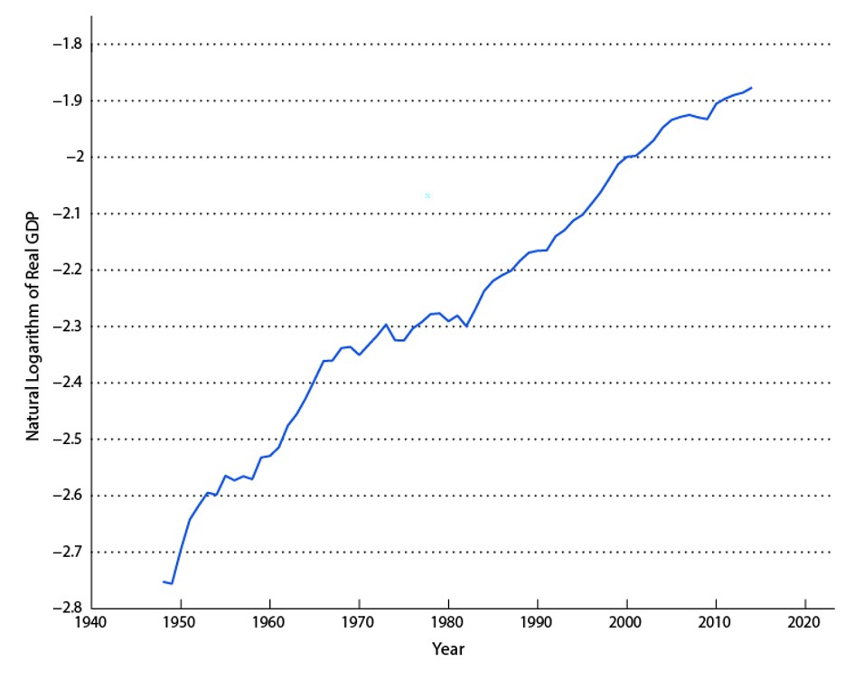
\includegraphics[scale=0.5]{Figures/W_Fig_7pt23.png}
%\end{figure}
%\end{frame}
%
%\begin{frame}
%\frametitle[alignment=center]{Growth Accounting}
%\begin{itemize}
%\item Read Williamson 7.7 and complete the updated exercise in the homework.
%\end{itemize}
%\end{frame}
%




\end{document}